%Vorlage fuer Thesen an der FFHS
\documentclass{ffhsthesis}

\usepackage[utf8]{inputenc}
\usepackage{amsmath}
\usepackage{algpseudocode}
\usepackage{algorithm}
\usepackage{amssymb}
\usepackage{tabularx}
\usepackage{hyperref}


\begin{document}


\dokumentTyp{Bachelor-Thesis}
\studiengang{INF}
\title{Optimierte Lagerverwaltungs-Strategie durch Reinforcement Learning}
%\subtitle{Optionaler Untertitel} % optional
%\titelbild[height=2cm,width=10cm]{ffhslogo}  % optional
\author{Benjamin Cirmena}
% \date{}
\wohnort{Kehrsatz}
%\referent{Name des Referenten\\ Titel\\Unterrichtetes Fach}
\referent{Dr.\ Beat Tödtli\\Dozent bei der FHS St.Gallen}
\eingereichtBei{Dr.\ Oliver Kamin\\Departement Informatik\\Departementsleiter} 

%\dedication{Diese Thesis widme ich meiner Verlobten, die mich während des gesamten Studiums tatkräftig unterstützt hat.}

\maketitle


\begin{zusammenfassung}
Lagerverwaltungssysteme benötigen durch die steigenden Anforderungen raffiniertere Strategien. Anpassungen in einem solchen System können einen grossen Einfluss auf die Strategie haben und würden daher eine Anpassung der Strategie benötigen. Mit Hilfe von Reinforcement Learning könnte eine solche Strategie selbstständig erlernt werden, welche möglicherweise die heuristische Strategie übertrifft.
In dieser Arbeit wird ein erweiterbares Environment aufgebaut, mit dem möglichst unterschiedliche Lagersysteme dargestellt werden können. Anschliessend werden zwei Experimente aufgebaut, um die Performanz der durch Reinforcement Learning erlernten Strategien mit der heuristischen Strategie zu vergleichen. In den Experimenten werden die beiden Reinforcement Learning-Algorithmen Sarsa und Q-Learning verwendet. Dabei wird die erreichte Performanz, der durchschnittlich erreichte Reward, mit der Performanz der heuristischen Strategie verglichen. Die Resultate haben gezeigt, dass die beiden Algorithmen in den beiden Experimenten die heuristische Strategie übertroffen haben.
\end{zusammenfassung}
\newpage
\begin{abstract}
Warehouse management systems require more sophisticated policies due to the increasing requirements. Adjustments in such a system can have a major impact on the policy and would therefore require policy adjustments. With the use of reinforcement learning, such a policy could be learned autonomously, which could possibly outperform the heuristic policy.
In this thesis an extensible environment is built, which allows to represent different storage systems. Subsequently, two experiments are set up to compare the performance of the strategies learned by reinforcement learning with the performance of the heuristic strategy. In the experiments the two reinforcement learning algorithms Sarsa and Q-Learning are used. The achieved performance, the average achieved reward, is compared with the performance of the heuristic strategy. The results showed that the two algorithms outperformed the heuristic strategy in both experiments.
\end{abstract}

\tableofcontents


\begin{abkuerzungen}[MUSTER] % Das Muster dient zur Bestimmung der Einrueckungstiefe
\item[RL] Reinforcement Learning
\item[MDP] Markov-Decision-Process
\item[MRP] Markov-Reward-Process
\item[MC] Monte-Carlo
\item[TD] Temporal-Difference
\end{abkuerzungen}


\startThesis % Befehl muss vor dem ersten chapter stehen (Seitennummerierung!)


\chapter{Einleitung}
Durch die Zunahme des Onlineshoppings und durch Next-Day oder sogar Same-Day-Lieferungen, steigen die Anforderungen an die Logistikprozesse im Hintergrund. Solche Logistikprozesse können komplex werden und müssen auch auf diverse Einflüsse reagieren können. 
Maschinelles Lernen könnte bei der Optimierung solcher Prozesse eine erhebliche Rolle spielen. Es gibt diverse algorithmische Ansätze, wobei in drei Gruppen aufgeteilt wird: überwachtes, unüberwachtes und bestärkendes Lernen. 
In dieser Thesis wird das bestärkende Lernen, auch Reinforcement Learning genannt, behandelt. Oft wird von Reinforcement Learning in Zusammenhang mit Spielen berichtet – sei es mit konventionellen Brettspielen wie Go oder Videospielen wie StarCraft. In dieser Arbeit wird überprüft, ob sich Reinforcement Learning eignet, um selbständig eine Policy zu erlernen, welche ein vereinfachtes Lager bewirtschaften kann (einlagern, bestellen, ausliefern). Des Weiteren soll aufgezeigt werden, ob sich Reinforcement Learning auch nach einer Skalierung des vereinfachten Beispiels immer noch eignet. Damit soll die Arbeit Aufschluss darüber geben, ob Reinforcement Learning auch in einem reellen Lager mit mehreren Tausend Artikeln funktionieren kann.
Jing-Sheng Song et al. \cite{inventory_management} haben prognostiziert, dass in Zukunft der Bedarf an Algorithmen, die in absehbarer Zeit die Abläufe einer Supply-Chain optimieren, immer stärker zunimmt. Es soll möglich sein, eine neue Anforderung festzulegen, sodass der Algorithmus selbständig sämtliche Teile der Supply-Chain optimiert. Die Mehrheit der Literatur befasst sich mit der Supply-Chain als Ganzes. So haben S. Kamal Chaharsooghi et al. \cite{rl_supply} erfolgreich eine Supply-Chain-Strategie durch Reinforcement Learning erlernt, die das Simulationsspiel «The Beergame App» mit einem zufriedenstellenden Ergebnis spielt. Das Warenhaus an sich wird dabei jedoch kaum betrachtet. In den Warenhäusern ist neben dem Optimieren der Bestell- und Lieferabläufe auch das Optimieren der Lagerung selbst interessant. Um ein Lager zu optimieren, müssen Strategien festgelegt werden, nach denen die Artikel eingelagert werden. Eine neue Paketgrösse kann unter Umständen zu einer Anpassung der gesamten Strategie führen. Des Weiteren wird es mit zunehmenden Faktoren, wie der Lagertemperatur von Artikeln oder der Beliebtheit eines Artikels, auf die die Strategie reagieren soll, immer schwieriger, eine passende Strategie zu definieren.

\section{Forschungsfragen}
\label{sec:ff}
In dieser Engineering-Arbeit werden folgende Forschungsfragen mithilfe einer entwickelten Simulationsumgebung, welche im \autoref{sec:warehouse} definiert ist, untersucht. Diese Umgebung entspricht auch dem Geltungsbereich.
\begin{itemize}
	\item \textbf{Forschungsfrage 1:}
\emph{Wie vergleicht sich die Performanz einer heuristischen Lagerverwaltungsstrategie mit einer durch Reinforcement Learning erlernten Strategie im zuvor definierten Environment?}
	\item \textbf{Forschungsfrage 2:}
\emph{Wie verhält sich die Performanz bei einer durch Reinforcement Learning erlernten Strategie mit einer zunehmenden Komplexität?}
\end{itemize}

\section{Abgrenzung und Vorgehensweise}
Diese Arbeit soll eine Grundlage für zukünftige Forschung bieten. Dabei wird der Fokus hauptsächlich auf die Lagerbewirtschaftung gelegt. Es wird ein vereinfachtes Environment erstellt, welches nur Basisfunktionen bietet. Des Weiteren wird in dieser Arbeit aus zeitlichen Gründen das Augenmerk auf grundlegende Algorithmen gerichtet. 
Um die beiden Forschungsfragen zu beantworten wird jeweils ein Experiment aufgebaut, welches die Performanz der Strategien mit dem durchschnittlich erhaltenen Reward vergleicht.
\section{Struktur der Arbeit}
Diese Arbeit ist wie folgt gegliedert: In Kapitel 2 wird eine Einführung ins Thema Reinforcement Learning gewährt, wobei der Fokus auf die grundlegenden Methoden und Algorithmen gelegt wird. In Kapitel 3 wird die das Environment definiert. In Kapitel 4 wird die angewendete Forschungsmethode beschrieben. In den Kapitel 5 und 6 werden die jeweiligen Experimente beschrieben, durchgeführt und die Resultate werden präsentiert. Anschliessend folgt in Kapitel 7 die Diskussion mit einem Ausblick auf weiterführende Arbeiten.
\chapter{Reinforcement Learning} 
Dieses Kapitel dient dazu, die Grundlagen von Reinforcement Learning zu erläutern. Dabei wird besonderer Fokus auf die Terminologie sowie auf grundlegende Konzepte und Algorithmen gelegt. 
Im Gegensatz zu anderen Machine-Learning-Gebieten wird beim Reinforcement Learning nicht zwingend mit verfügbaren Daten gearbeitet. Die benötigten Informationen werden durch ‹Trial-and-Error› generiert. Ein sogenannter Agent führt in einer Simulationsumgebung, dem Environment, Handlungen aus. Diese Handlungen werden Actions genannt. 
 

 \begin{figure}[ht]
  \centering
  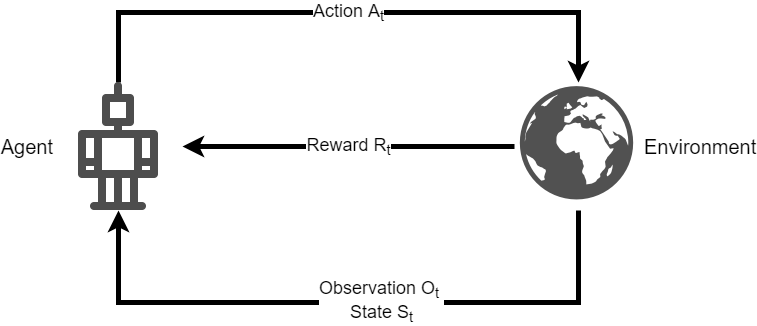
\includegraphics[height=4.5cm]{img/RL_Agent_Env.png}
  \label{rl_draw}
  \caption{RL-Agent und Environment}
\end{figure}

Nach jeder Action erhält der Agent einen Reward und eine Observation. Der Reward informiert den Agent, wie gut seine Action war. Dabei kann der Reward sowohl positiv als auch negativ sein. Die Wahl des Rewards hängt vom Environment und dem Task ab. Er könnte dem gewonnenen Score in einem Spiel entsprechen, einem Börsen-Kurs oder einem vordefinierten Wert für gewisse Umstände im Environment. Daneben erhält der Agent auch eine Observation. Die Observation enthält Informationen aus dem State des Environments. In einer perfekten Welt umfasst die Observation den gesamten Space des Environments. In diesem Fall würde der State im Agent dem des Environments entsprechen. Wenn in Reinforcement Learning vom State gesprochen wird, ist im Normalfall die Rede vom internen State des Agents. Das Ziel des Agents ist es, den gesamten Reward zu maximieren.

\section{Markov-Prozess}
Reinforcement Learning setzt voraus, dass Entscheidungen in einem Environment nach dem Markov-Decision-Process (MDP) getroffen werden. Jedes Environment handelt nach einem MDP. In den folgenden Kapiteln werden die Bestandteile, welche einen MDP ausmachen, beschrieben. Dadurch soll ein Verständnis aufgebaut werden, wie ein MDP gelöst werden kann. Ein MDP setzt die Markov-Eigenschaft voraus. Diese Eigenschafft ist erfüllt, wenn in einem stochastischen Prozess die Wahrscheinlichkeitsverteilung für zukünftige States nur vom aktuellen State abhängig ist und nicht von der Vergangenheit. Jede Umgebung kann grundsätzlich als MDP definiert werden; dazu müssen nur genügend Informationen im State vorhanden sein, welcher unter Umständen auch die Vergangenheit selbst beinhaltet.

\begin{equation}
\mathbb{P}[S_{t+1}\ |\ S_t]=\ \mathbb{P}[S_{t+1}\ |\ S_1,\ \ldots,\ S_t]
\end{equation}

Aufbauend auf dieser Eigenschaft entsteht ein Markov-Prozess. Dieser Prozess ist eine Sequenz von zufälligen States, welche die Markov-Eigenschaft haben. Der Markov-Prozess ist ein Tupel aus $\mathcal{S}$, dem State-Space, einer endlichen Anzahl möglicher States und $\mathcal{P}$, der Übergangsmatrix, welche für jeden State-Übergang die Wahrscheinlichkeit beschreibt. Anhand dieser Tupel kann eine Kopie des Environments erstellt werden, welche genau gleich auf die States reagiert.


 \begin{figure}[ht]
 \centering
  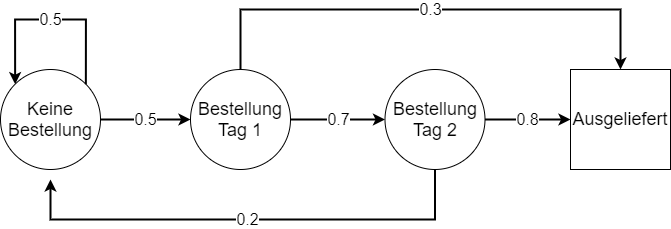
\includegraphics[height=5cm]{img/Markov_Prozess_Ext.png}
  \caption{Markov-Prozess}
  \label{mp_draw}
\end{figure}


Das Beispiel in Abbildung \ref{mp_draw} zeigt einen solchen Markov-Prozess auf. Im Status «Keine Bestellung» besteht eine Übergangswahrscheinlichkeit von 50 Prozent, dass eine neue Stellung eintrifft. Ist eine Bestellung eingetroffen, besteht die Wahrscheinlichkeit von 30 Prozent, dass der Artikel bereits vorhanden ist und direkt ausgeliefert wird. Wurde die Bestellung nicht ausgeliefert, so besteht am nächsten Tag erneut eine Wahrscheinlichkeit, dass der Artikel nun vorhanden ist und ausgeliefert wird. Ist das nicht der Fall, annulliert in diesem Beispiel der Kunde die Bestellung.

\section{Markov Reward Process}
Der Markov-Reward-Process (MRP) baut auf dem Markov-Prozess auf und fügt eine Wertung der Übergänge hinzu. Der MRP wird durch die Tupel $\langle S,P,R,\gamma \rangle$ beschrieben. Dabei steht $\mathcal{R}$ für die Reward-Funktion; diese beschreibt, welcher State welchen Reward erhält. 

 \begin{figure}[ht]
  \centering
  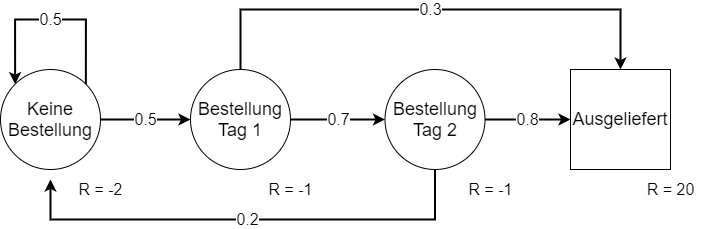
\includegraphics[height=5cm]{img/Markov_Reward_Prozess.png}
  \caption{Markov-Reward-Process}
  \label{mrp_draw}
\end{figure}

Der Discount-Factor $\gamma$ beschreibt, wie stark zukünftige Rewards gewichtet werden. Ein Discount-Factor von 1 beachtet alle zukünftigen Rewards und ein Discount-Factor von 0 betrachtet nur den aktuellen Reward. Das Ziel in einem MRP ist es, den Return $G_t$, den gesamten diskontierten Reward eines Zeitschritts $t$, zu maximieren.

\begin{equation}
    G_t=R_{t+1}+{\gamma R}_{t+2}+{\gamma^2R}_{t+3}+...\ =\sum_{k=0}^{\infty}{\gamma^kR}_{t+k+1}
\end{equation}

\newpage
Um den Return genauer zu veranschaulichen, folgen nun einige mögliche Sequenzen des MRPs aus Abbildung \ref{mrp_draw}. Es wird ein Discount-Factor von 0.5 verwendet und die Sequenzen starten beim State «Keine Bestellung».



\begin{align}
    &\boldsymbol{KB\xrightarrow{}BT1\xrightarrow{}A}\nonumber\\
    &v=-2+(-1\ast\frac{1}{2})+(20\ast\frac{1}{4})\ =2.5\\ \nonumber\\
    &\boldsymbol{KB\xrightarrow{}BT1\xrightarrow{}BT2\xrightarrow{}A}\nonumber\\
    &v=-2+(-1\ast\frac{1}{2})+(-1\ast\frac{1}{4})+(20\ast\frac{1}{8})\ =-0.25\\ \nonumber\\
    &\boldsymbol{KB\xrightarrow{}BT1\xrightarrow{}BT2\xrightarrow{}KB\xrightarrow{}KB\xrightarrow{}BT1\xrightarrow{}A}\nonumber\\
    &v=-2+(-1\ast\frac{1}{2})+(-1\ast\frac{1}{4})+(-2\ast\frac{1}{8})+(-2\ast\frac{1}{16})+(-1\ast\frac{1}{32})+(20\ast\frac{1}{64}) \nonumber\\
    &v=-\frac{91}{32}\approx-2.84
\end{align}



\section{Bellman-Expectation-Equation}
Die Value-Function wertet einen gegebenen State aus. Dabei wird der erwartete Return für den entsprechenden State berechnet. 




\begin{align}
&v(s)\ =\ \mathbb{E}\ [G_t\ |{\ S}_t=s] \nonumber\\
&v(s)\ =\ \mathbb{E}\ [R_{t+1}+{\gamma G}_{t+1}\ |{\ S}_t=s] \nonumber\\
&v(s)\ =\ \mathbb{E}\ [R_{t+1}+{\gamma v(S}_{t+1})\ |{\ S}_t=s] \label{bellman-exp-equa}
\end{align}


Bei der Value-Function handelt es sich um eine rekursive Gleichung, wobei der Wert der aktuellen States aus dem zu erwartenden Reward und dem diskontierten Wert des folgenden States besteht. Dies entspricht der Bellman-Expectation-Equation; diese kann auch als Matrixrepräsentation dargestellt werden.
\begin{equation}
  v=\mathcal{R}+\gamma\mathcal{P}v
\end{equation}

\begin{equation}
\left[\begin{matrix}v(1)\\\vdots\\v(n)\\\end{matrix}\right]\ =\left[\begin{matrix}\mathcal{R}_1\\\vdots\\\mathcal{R}_n\\\end{matrix}\right]\left[\begin{matrix}\mathcal{P}_{11}&\cdots&\mathcal{P}_{1n}\\\vdots&\ddots&\vdots\\\mathcal{P}_{n1}&\cdots&\mathcal{P}_{nn}\\\end{matrix}\right]\left[\begin{matrix}v(1)\\\vdots\\v(n)\\\end{matrix}\right]
\end{equation}


Diese lineare Gleichung kann direkt gelöst werden:
\begin{align}
 v&=\mathcal{R}+\gamma\mathcal{P}v \nonumber\\
\left(I-\gamma\mathcal{P}\right)\ v&=\mathcal{R} \nonumber\\
v&=\left(I-\gamma\mathcal{P}\right)^{-1}\ \mathcal{R} \label{solve-lin-equa}
\end{align}



Dabei ist zu beachten, dass diese Variante nur für kleine MRPs geeignet ist, da die Zeitkomplexität für diese Berechnung $0(n^3)$ beträgt, wobei n für die Anzahl States steht. Für grössere MRPs gibt es erweiterte Methoden, welche noch in den folgenden Kapiteln erläutert werden. Nun kann diese Formel am MRP aus dem vorherigen Beispiel angewendet werden. In diesem Beispiel wird ein Discount-Factor von 1 verwendet, womit alle zukünftigen Returns berücksichtigt werden.

\begin{equation}
  \left(\left[\begin{matrix}\begin{matrix}1&0\\0&1\\\end{matrix}&\begin{matrix}0&0\\0&0\\\end{matrix}\\\begin{matrix}0&0\\0&0\\\end{matrix}&\begin{matrix}1&0\\0&1\\\end{matrix}\\\end{matrix}\right]-1\left[\begin{matrix}\begin{matrix}0.5&0.5\\0&0\\\end{matrix}&\begin{matrix}0&0\\0.7&0.3\\\end{matrix}\\\begin{matrix}0.2&0\\0&0\\\end{matrix}&\begin{matrix}0&0.8\\0&0\\\end{matrix}\\\end{matrix}\right]\right)^{-1}\left[\begin{matrix}\begin{matrix}-2\\-1\\\end{matrix}\\\begin{matrix}-1\\20\\\end{matrix}\\\end{matrix}\right]=\left[\begin{matrix}\begin{matrix}13.37\\17.37\\\end{matrix}\\\begin{matrix}17.67\\20\\\end{matrix}\\\end{matrix}\right]  
\end{equation}


In der folgenden Abbildung ist der MRP mit den Values der jeweiligen States ersichtlich.
 \begin{figure}[h]
  \centering
  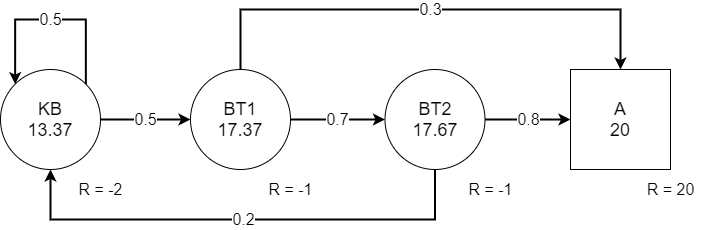
\includegraphics[width=\textwidth]{img/Bellman_Expectation_Equation.png}
  \caption{MRP mit Values}
\end{figure}

Ob diese Values stimmen, kann nun problemlos mit einem vorausschauenden Schritt in einem beliebigen State überprüft werden. Die Zahlen wurden auf zwei Kommastellen gerundet.


\begin{align}
&v(BT2) = \mathbb{E} [G_t |{ S}_t=s] \nonumber\\
\begin{split}
v(BT2) =R_{t+1}+ \gamma v(KB)\ast P(KB)+ \gamma v(BT1)\ast P(BT1) \\
+ \gamma v(BT2)\ast P(BT2)+\gamma v(A)\ast P(A) 
\end{split}\nonumber\\ 
&v(BT2) =-1+ 13.37\ast0.2+ 17.37\ast0+ 17.67\ast0+20\ast0.8 \nonumber\\
&v(BT2) = 17.67 \label{calculate-mrp}
\end{align}


		
\section{Markov-Decision-Process}
Der Markov-Decision-Process (MDP) erweitert den MRP um $\mathcal{A}$, eine endliche Anzahl möglicher Actions. Somit wird der MDP mit dem folgenden Tupel definiert $\langle S,A,P,R,\gamma \rangle$.  Dabei wird die Übergangsmatrix $\mathcal{P}$ mit der jeweiligen Action erweitert und beschreibt somit die Wahrscheinlichkeit der State-Action-Übergänge. Auch die Reward-Funktion $\mathcal{R}$ benötigt zusätzlich eine Action, um den Reward zu berechnen. Da nun die State-Übergänge durch Actions beeinflusst werden, muss die Value-Function angepasst werden. Die Value-Function wird nun so angepasst, dass sie einer Strategie, einer sogenannten Policy $\pi$, folgt. Eine solche Policy beschreibt für einen State S, mit welcher Wahrscheinlichkeit die möglichen Actions gewählt werden. Die Value-Function $v_\pi(S)$ beschreibt den Wert eines States – vorausgesetzt, die zukünftigen Actions werden nach der Policy $\pi$ gewählt. 

\begin{equation}
v_\pi(S)\ ={\ \mathbb{E}}_\pi\ [R_{t+1}+{\gamma v_\pi(S}_{t+1})\ |{\ S}_t=s]
\end{equation}

Um einen MDP zu lösen und eine optimale Policy zu finden, muss unterschieden werden, ob das Model bekannt ist, welches das Environment beschriebt – also die kompletten Tupel, die den MDP beschreiben. Oft sind nicht alle Dynamiken eines Environments bekannt oder die Menge an zu verarbeitenden Informationen ist nicht mehr geeignet.

In Abbildung \ref{fig:mdp} wird erneut das Lagerbeispiel verwendet. Die States wurden zudem mit der Information erweitert, ob ein Artikel auf Lager ist oder nicht. Ausserdem verfügt nun der Agent über drei verschiedene Actions: A1 – \emph{Warten}, A2 – \emph{Beim Lieferanten bestellen} und A3 – \emph{Ausliefern}. Die drei Kreuzungen zwischen den States stellen die probabilistischen Ausgänge aus den jeweiligen Actions dar. Falls in diesem Beispiel ein Artikel beim Lieferanten bestellt wird, so ist dieser garantiert am nächsten Tag da. Die Wahrscheinlichkeit, dass am nächsten Tag eine neue Bestellung von einem Kunden eintrifft, ist nur 50 Prozent.

 \begin{figure}[h]
  \centering
  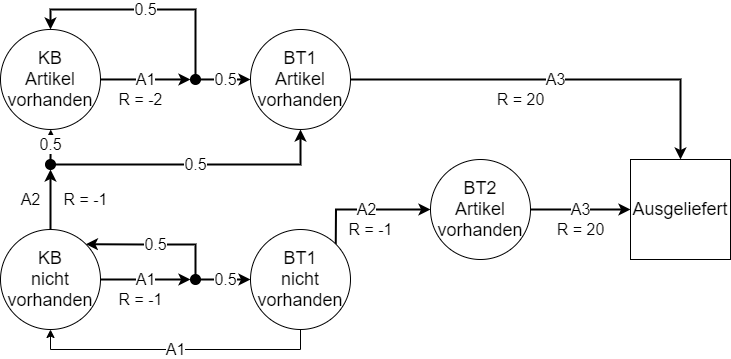
\includegraphics[width=\textwidth]{img/Markov_Decision_Prozess.png}
  \caption{Markov-Decision-Process}
  \label{fig:mdp}
\end{figure}




\section{Bellman-Optimality-Equation}
Anders als bei der Bellman-Expectation-Equation, die bereits zum Evaluieren der Value-Function einer bestimmten Policy benötigt wird, ist die Bellman-Optimality-Equation keine lineare Gleichung. Wenn in der Literatur von der Bellman-Equation die Rede ist und nicht weiter spezifiziert wird, betrifft es meistens die Bellman-Optimality-Equation. Das Ziel dieser Gleichung ist es nicht, den Wert eines States bei einer definierten Policy $\pi$ zu evaluieren, sondern eine optimale Policy $\ast$ zu finden. 

\begin{align}
&v_\ast(s)\ =\max_\pi{v_\pi}(s) \nonumber\\
&v_\ast(s)\ =\max_a{\mathcal{R}(s,a)}+\gamma\sum_{S^\prime}{\mathcal{P}(s,a,s^\prime)}v_\ast(s^\prime) \label{bellman-opt-equa}
\end{align}


\newpage
Dabei wird bei der optimalen State-Value-Function nicht die optimale Policy gesucht, sondern der maximal mögliche Reward, welcher der Agent aus einem Environment bekommen kann. Im Beispiel des MDP würden bei einem Discount-Factor von 1 folgende Values errechnet (Anhang \ref{appendix:state-values}):

\begin{figure}[ht]
  \centering
  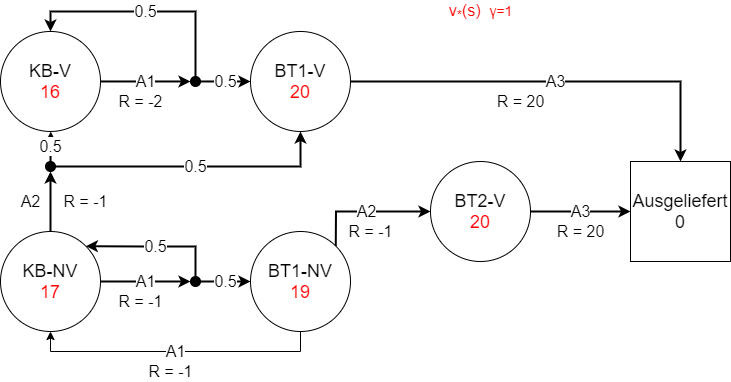
\includegraphics[width=\textwidth]{img/MDP_State-Value_Function.png}
  \caption{MDP-State-Value-Function}
    \label{fig:mdp-value}
\end{figure}
Um die optimale Policy zu finden, welche den MDP komplett löst, wird die optimale Action-Value Function benötigt.
\begin{align}
&q_\ast\left(s,a\right)=\max_\pi{q_\pi}\left(s,a\right) \nonumber\\
&q_\ast(s,a)\ =\mathcal{R}(s,a)+\gamma\sum_{S^\prime}{\mathcal{P}(s,a,s^\prime)}{max\ {q_\ast}_{a^\prime}(s^\prime,a^\prime)} \label{bellman-opt-equa-q}
\end{align}

\newpage
Die optimale Action-State-Function sagt für einen State und eine Action aus, welches der maximale zukünftige Reward für die aktuelle Situation ist. Die entsprechenden Q-Values für diese optimale Policy wurde im Anhang \ref{appendix:action-values} berechnet.
 \begin{figure}[H]
  \centering
  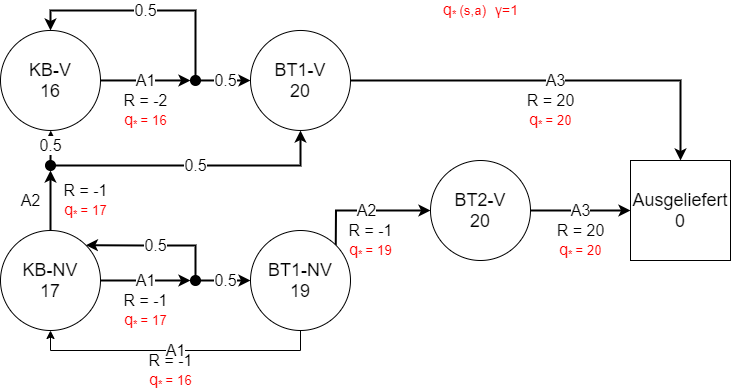
\includegraphics[width=\textwidth]{img/MDP_Action-Value_Function.png}
  \caption{MDP-Action-Value-Function}
      \label{fig:mdp-action-value}
\end{figure}

Betrachtet man in diesem Beispiel (Abbildung \ref{fig:mdp-action-value}) den Start-State «KB-NV», so wird nun klar, dass der maximal mögliche Reward 17 ist, egal ob die Action A1 – \emph{Warten} oder die Action A2 – \emph{Beim Lieferanten bestellen} ausgeführt wird. Mit diesen Q-Values der optimalen Policy können nun die Actions in diesem MDP immer optimal gewählt werden. Ein MDP hat zwingend mindestens eine deterministisch optimale Policy.


\section{Model-free Prediction}
Bei der Model-free Prediction kennt der Agent das Model des MDP nicht. Der Agent sammelt Informationen über das Environment und versucht so, seine aktuelle Policy zu evaluieren. Dazu gibt es diverse Methoden, welche aber im Grundsatz auf den folgenden beiden Methoden aufbauen.
\subsection{Monte-Carlo-Learning}
Die Monte-Carlo(MC)-Methode evaluiert eine Policy anhand der Erfahrung ganzer Episoden. Eine Episode stellt eine Sequenz an Actions dar, die in einem Environment durchgeführt werden. Diese Durchführung von Actions geschieht so lange, bis ein Abbruchkriterium erreicht ist und somit die Episode beendet wurde. Der Agent führt eine bestimmte Sequenz lang Actions nach der Policy durch, bis die Episode beendet wird. Dabei wird eine Anzahl an Episoden festgelegt, die der Agent durchläuft. Bei dieser Methode benötigt der Agent zwingend die kompletten Episoden zum Evaluieren. Der Agent durchläuft dabei die Episoden, nimmt den jeweiligen Return und berechnet den durchschnittlichen Return für alle Episoden. Der dabei berechnete empirische Return konvergiert mit steigender Anzahl der Episoden gegen den zu erwartenden Return. Somit nähert sich auch die Value-Function der tatsächlichen Value-Function an.
\subsection{Temporal-Difference-Learning}
Im Gegensatz zur MC-Methode evaluiert die Temporal-Difference(TD)-Methode eine Policy nicht mit der Erfahrung aus einer kompletten Episode, sondern aus einer Schätzung, welche aus einer Sequenz von Actions durchgeführt wurde. Es wird eine bestimmte Anzahl $n$ Actions durchgeführt, mit welchen anschliessend eine Schätzung für den Return durchgeführt wird. Daraufhin wird nach den nächsten n Actions die Schätzung der Values mit der neuen Schätzung des Returns aktualisiert. Dieses Vorgehen wird Bootstrapping genannt, da eine Schätzung aufgrund einer anderen Schätzung durchgeführt wird.

 \begin{figure}[ht]
  \centering
  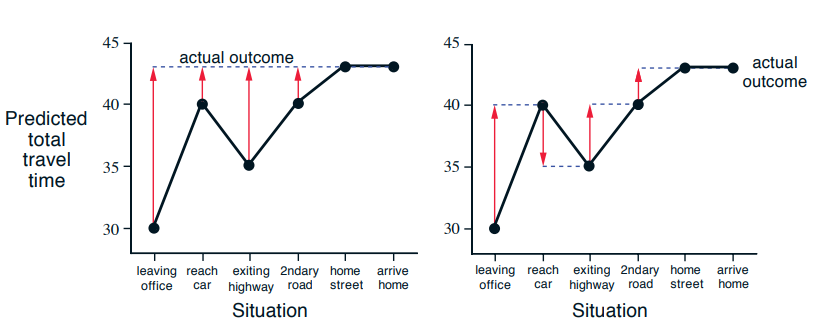
\includegraphics[width=\textwidth]{img/diff_mc_td.png}
  \caption{Unterschied MC \& TD \cite{td-mc}}
      \label{fig:diff-mc-td}
\end{figure} 


\newpage
\section{Model-free Control}
Ist das Model eines MDPs bekannt und der Agent kennt die Übergangswahrscheinlichkeiten sowie die Reward-Funktion des MDPs, so kann mittels Dynamic-Programming und Policy-Iteration die optimale Policy erlernt werden. Oft ist in der Realität bei Problemstellungen, in denen Reinforcement Learning angewendet wird, kein Model bekannt, welches den genauen MDP beschreibt. Daher muss der Agent wie in der Model-free Prediction mithilfe gemachter Erfahrungen die aktuell angewendete Policy evaluieren und verbessern. Zur Verbesserung einer Policy ist ein gewisses Mass an Exploration nötig. Ein Agent, welcher nicht exploriert, sondern nur exploitiert, wählt die aus seiner aktuellen Policy beste Action. Stellt man sich ein minimales Beispiel vor, in dem eine Action im aktuellen State einen Reward von 2 ergibt und die andere einen Reward von 10, wird – sofern die erwarteten Returns mit 0 initialisiert wurden und somit beide einen gleichen erwarteten Return haben – eine zufällige erste Action gewählt. Bei der Wahl einer Action, welche einen Reward von 2 ergibt, wird ohne Exploration nie eine andere Action ausprobiert und der Reward von 10 würde somit nie erreicht werden. 
\subsection{Epsilon-greedy Exploration}
Die Epsilon-greedy Exploration ist eine oft verwendete Methode, um sicherzustellen, dass der Agent neue Actions ausprobiert und somit das ganze Environment kennenlernt. So kann er die bestmögliche Policy finden. Dabei wird ein Wert $\epsilon$ (Epsilon) zwischen 0 und 1 festgelegt. Vor jeder Action wird mit der Wahrscheinlichkeit 1 - $\epsilon$ die beste Action, die Greedy Action ausgeführt. Mit der Wahrscheinlichkeit $\epsilon$ wird eine zufällige Action ausgeführt. Würden unendlich viele Schritte durchgeführt, so würde jedes State-Action-Paar unendlich oft besucht werden. Somit kann ausgeschlossen werden, dass eine bestimmte Policy nicht entdeckt wird.

\begin{equation}
   \pi(a|s)
\left\{\begin{matrix}
 1-\epsilon,&  \underset{a\in A} {\mathrm{argmax}} ~Q(s,a)\\ 
 \epsilon,& random(a)
\end{matrix}\right. 
\end{equation}

Ein Nachteil bei der Epsilon-greedy Exploration ist, dass die Policy nie wirklich mit der optimalen Policy konvergiert, da weiterhin zufällig Actions ausgeführt werden. Eine Möglichkeit, dem entgegenzuwirken, besteht darin, $\epsilon$ über die Zeit zu verkleinern.




\subsection{Sarsa}
Der Sarsa-Algorithmus \cite{rummery1994line} basiert auf dem Prinzip der TD. Dabei wird in einem State-Action-Paar gestartet. Der Agent erhält ein Reward und erreicht einen neuen State. Nun nimmt der Agent seine Schätzung für das folgende State-Action-Paar der Policy; dieser diskontierte Q-Value zusammen mit dem Reward muss laut der Bellman-Equation dem vorherigen Q-Value entsprechen. Der Ausgangs-Q-Value $Q\left(S,A\right)$ wird anhand der Lernrate $\alpha$ in Richtung TD-Target korrigiert (\ref{sarsa_eq}). Die Differenz zwischen TD-Target und dem Ausgangs-Q-Value ist der TD-Error; dieser muss bei einer Greedy Policy konvergieren, sonst wurde keine optimale Policy gefunden. 

 \begin{figure}[ht]
  \centering
  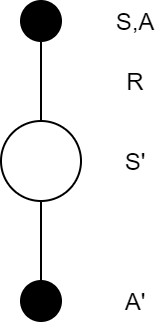
\includegraphics[height=3cm]{img/SARSA (1).png}
  \caption{Sarsa-Update}
      \label{fig:sarsa-update}
\end{figure} 

\begin{align}
&Q\left(S,A\right)\gets Q\left(S,A\right)+\alpha\left(R+\gamma Q\left(S^\prime,A^\prime\right)-Q\left(S,A\right)\right) \nonumber\\
&Q\left(S,A\right)\gets Q\left(S,A\right)+\alpha\left(TDTarget-Q\left(S,A\right)\right) \nonumber\\
&Q\left(S,A\right)\gets Q\left(S,A\right)+\alpha\left(TDError\right) \label{sarsa_eq}
\end{align}




\begin{algorithm}
\begin{algorithmic}[1]
\State{Algorithm parameters: step size $\alpha \in$ (0, 1), small $\epsilon$ > 0}
\State{Initialize  $Q(s,a)$, for all $s\in S^+,a\in A(s)$, arbitrarily except that $Q(terminal)$=0}
\Repeat { for each episode}
\State{Initialize $S$}
\State{Choose $A$ from $S$ using policy derived from $Q$ (e.g., $\epsilon$-greedy)}
  \Repeat{ for each step of episode}
    \State {Take action $A$, observe $R$, $S'$}
    \State {Choose $A'$ from $S'$ using policy derived from $Q'$ (e.g., $\epsilon$-greedy)}
    \State {$Q(S,A)\gets Q(S,A)+ \alpha [R+ \gamma Q(S',A') -Q(S,A)]$}
    \State {$S\gets S'; A \gets A';$}
    \Until{$S$ is terminal}
\end{algorithmic}
\caption{Sarsa-Algorithmus \cite{sutton_reinforcement_2018} Chapter 6}
\end{algorithm}




\subsection{Q-Learning}
Im Gegensatz zu Sarsa ist Q-Learning \cite{dayan1992q, watkins1989learning} ein Off-Policy-Algorithmus. Das bedeutet, der Agent wählt zwar – wie bei Sarsa – eine Action nach der Epsilon-greedy Policy, nimmt aber für die Schätzung die Action nach der Greedy Policy. Dieses Vorgehen entspricht dem Prinzip der Bellman-Optimality-Equation.

 \begin{figure}[ht]
  \centering
  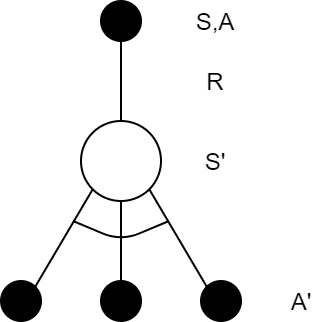
\includegraphics[height=3cm]{img/Q-Learning.png}
  \caption{Q-Learning-Update}
      \label{fig:q-update}
\end{figure} 








\begin{equation}
    Q\left(S,A\right)\gets Q\left(S,A\right)+\alpha\left(R+\gamma\max_{a^\prime}
{Q\left(S^\prime,a^\prime\right)}-Q\left(S,A\right)\right)
\end{equation}


\begin{algorithm}
\begin{algorithmic}[1]
\State{Algorithm parameters: step size $\alpha \in$ (0, 1), small $\epsilon$ > 0}
\State{Initialize  $Q(s,a)$, for all $s\in S^+,a\in A(s)$, arbitrarily except that $Q(terminal)$=0}
\Repeat { for each episode}
\State{Initialize $S$}
  \Repeat{ for each step of episode}
    \State{Choose $A$ from $S$ using policy derived from $Q$ (e.g., $\epsilon$-greedy)}
    \State {Take action $A$, observe $R$, $S'$}
    \State {$Q(S,A)\gets Q(S,A)+ \alpha [R+ \gamma max_a Q(S',a) -Q(S,A)]$}
    \State {$S\gets S'$}
    \Until{$S$ is terminal}
\end{algorithmic}
\caption{Q-Learning-Algorithmus \cite{sutton_reinforcement_2018} Chapter 6}
\end{algorithm} 
\chapter{Environment}
Um die Forschungsfragen dieser Thesis zu beantworten, ist ein Environment nötig, welches auf minimale Weise Prozesse in einem Lager abbildet. Dabei soll das Environment so aufgebaut werden, dass ein Agent lernen muss, möglichst wenige Artikel am Lager zu halten, damit Kosten eingespart werden. Des Weiteren müssen wiederum genügend Artikel gelagert sein, sodass keine Lieferfrist vergeht und somit ein Auftrag storniert wird. Dieses Environment soll dabei möglichst erweiterbar aufgebaut werden und dem gängigen Standard von Reinforcement Learning Environments entsprechen. Dadurch wird sichergestellt, dass ohne grossen Aufwand verschiedene Algorithmen überprüft werden können.
\section{OpenAI Gym}
OpenAI, ein Unternehmen, welches sich mit der Erforschung von künstlicher Intelligenz beschäftigt, hat mit Gym \cite{gym} einen Standard für Reinforcement Learning geschaffen. Dabei war es ihr Ziel, eine Library an Environments zur Verfügung zu stellen, um Algorithmen einfacher über verschiedene Situationen zu benchmarken. Hierzu wurde darauf geachtet, dass das Aufsetzen eines Environments ohne grossen Aufwand möglich ist und somit auch die Reproduzierbarkeit veröffentlichter Forschung erleichtert wird.
\subsection{Gym-Methoden}
OpenAI Gym sollte folgende Methoden umfassen:
\begin{itemize}
    \item \textbf{step():} Diese Methode startet einen Zeitschritt im Environment, wobei die auszuführende Action übergeben wird. Der Rückgabe-Wert dieser Funktion enthält immer eine Observation vom Typ «object», ein Reward vom Typ «float», ein Flag vom Typ «boolean», welches bestimmt, ob die aktuelle Sequenz in einem Terminalstatus angekommen ist, sowie zusätzliche Debug-Informationen vom Typ «dict», welche für den Agent nicht sichtbar sein sollten. 
\item \textbf{render():} Diese optionale Methode ermöglicht es, mit dem Gym-integrierten Viewer ein Frame vom Environment zu rendern.
\item \textbf{reset():} Diese Methode setzt den aktuellen Status im Environment auf den Start zurück. Dabei wird hier auch eine erste Observation zurückgegeben. Reset wird im Normalfall zu Beginn und nach dem «\emph{done}»-Flag nach jeder Sequenz ausgeführt.

\end{itemize}








\subsection{Gym-Attribute}
Folgende Attribute müssen im Gym enthalten sein:
\begin{itemize}
    \item \textbf{observation\_space:} Dieses Attribut widerspiegelt den observierbaren State-Space. Dabei kann es ein Objekt sein, welches dasselbe Format hat wie die Observationen aus den reset()- und step()-Methoden oder eine Instanz der Klasse Space, welche von OpenAI zur Verfügung gestellt wird.
    \item \textbf{action\_space:} Dieses Attribut kann ein Array von möglichen Actions sein oder auch eine Instanz der Klasse Space.
\end{itemize}


\section{WarehouseEnv}
\label{sec:warehouse}
Beim erstellten «WarehouseEnv» handelt es sich um ein Environment, welches einen terminalen State hat. Jede Episode hat genau 100 Zeitschritte, sogenannte Steps. 

\begin{figure}[ht]
  \centering
  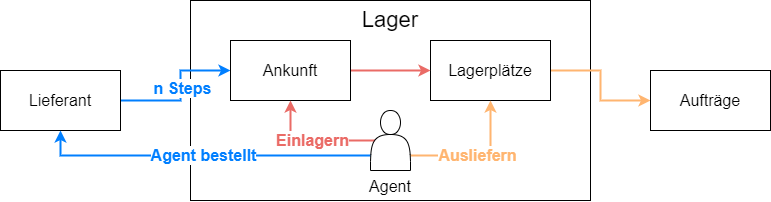
\includegraphics[width=\textwidth]{img/warehouse-env.png}
  \caption{WarehouseEnv}
    \label{fig:warehouse-env}
\end{figure} 

\newpage
\subsection{Environment-Step}
In jedem Step wird zuerst das Environment aktualisiert. Dabei wird überprüft, ob Aufträge storniert wurden und ob eine Bestellung im Wareneingang angekommen ist. Die Rewards dieser beiden Überprüfungen sowie ein Reward für die Lagerkosten werden nun vorgemerkt. Anschliessend findet die eigentliche Action statt; diese wird im Environment durchgeführt. Der Reward, welcher sich aus dem direkten Reward der Action sowie dem Reward der Aktualisierung ergibt, wird berechnet. Der Agent erhält nun eine Observation aus dem State und den Reward des durchgeführten Steps. \smallskip

\noindent\textbf{Lagerkosten}
\begin{table}[H]%
\begin{tabularx}{\textwidth} { 
  | >{\raggedright\arraybackslash}l 
  | >{\raggedright\arraybackslash}X | }
 \hline
 Reward &Dieser Reward wird vor jeder Aktion verteilt. Er ist abhängig vom genutzten Lagerplatz und soll somit Lagerkosten simulieren.\\
        &\textbf{-10 * Anzahl benutzter Lagerplätze}\\
\hline
\end{tabularx}
\caption{Lagerkosten}
\end{table}%

\noindent\textbf{Stornierter Auftrag}
\begin{table}[H]%
\begin{tabularx}{\textwidth} { 
  | >{\raggedright\arraybackslash}l 
  | >{\raggedright\arraybackslash}X | }
 \hline
 Reward &Dieser Reward wird vor jeder Aktion verteilt. Wird ein Auftrag storniert, so wird ein Reward von \textbf{-50} hinzugefügt.\\
\hline
\end{tabularx}
\caption{Stornierter Auftrag}
\end{table}%
\noindent\textbf{Bestellungseingang}
\begin{table}[ht]%
\begin{tabularx}{\textwidth} { 
  | >{\raggedright\arraybackslash}l 
  | >{\raggedright\arraybackslash}X | }
 \hline
 Reward	&Der Reward ist davon abhängig, ob im Wareneingang ein Platz frei ist.\\
&Artikel angekommen: \textbf{0}\\
&Artikel verworfen: \textbf{-25}\\
\hline
\end{tabularx}
\caption{Bestellungseingang}
\end{table}%

\newpage
\subsection{State-Space}
\label{sec:state-space}
Der State-Space besteht aus sämtlichen Entitäten und deren möglichen Zuständen. Die Anzahl der Entitäten sind jeweils Konstanten, welche im Environment festgelegt werden.
\noindent\textbf{Lagerplätze}
\begin{table}[H]%
\begin{tabularx}{\textwidth} { 
  | >{\raggedright\arraybackslash}l 
  | >{\raggedright\arraybackslash}X 
  | >{\raggedright\arraybackslash}l
  | >{\raggedright\arraybackslash}l|}
 \hline
  Anzahl &Anzahl der möglichen Lagerplätze &INT (const) &3\\
\hline
 Artikel &Pro Lagerplatz kann genau ein Artikel gelagert werden. &Artikel &Instanz\\
 \hline
\end{tabularx}
\caption{Lagerplätze}
\end{table}%
\noindent\textbf{Artikel}
\begin{table}[H]%
\smallskip
\begin{tabularx}{\textwidth} { 
  | >{\raggedright\arraybackslash}l 
  | >{\raggedright\arraybackslash}X 
  | >{\raggedright\arraybackslash}l
  | >{\raggedright\arraybackslash}l|}
 \hline
  Anzahl &Anzahl der möglichen Artikel &INT (const) &1\\
\hline
 Häufigkeit &Die Häufigkeit definiert, mit welcher Wahrscheinlichkeit ein Artikel bestellt wird. &FLOAT &[0-1]\\
 \hline
\end{tabularx}
\caption{Artikel}
\end{table}%

\noindent\textbf{Aufträge}\\
Sofern nicht die maximale Anzahl an Aufträgen ansteht, wird nach jedem vierten Step ein neuer Auftrag generiert. Dabei wird der Artikel nach der Artikelhäufigkeit gewählt. Ein Auftrag hat ausserdem eine Frist von 5 Steps. Wurde der Auftrag nicht ausgeliefert und somit abgeschlossen, so wird dieser vom Auftraggeber storniert.
\begin{table}[H]%
\begin{tabularx}{\textwidth} { 
  | >{\raggedright\arraybackslash}l 
  | >{\raggedright\arraybackslash}X 
  | >{\raggedright\arraybackslash}l
  | >{\raggedright\arraybackslash}l|}
 \hline
  Anzahl &Maximale Anzahl anstehender Aufträge &INT (const) &2\\
\hline
 Artikel &Jeder Auftrag enthält genau einen Artikel.  &Artikel &Instanz\\
 \hline
\end{tabularx}
\caption{Aufträge}
\end{table}%

\noindent\textbf{Wareneingang}\\
Die Artikel, die beim Hersteller bestellt wurden, erscheinen nach der Lieferzeit von zwei Steps im Wareneingang. 
\begin{table}[H]%
\begin{tabularx}{\textwidth} { 
  | >{\raggedright\arraybackslash}l 
  | >{\raggedright\arraybackslash}X 
  | >{\raggedright\arraybackslash}l
  | >{\raggedright\arraybackslash}l|}
 \hline
  Anzahl &Anzahl der Plätze im Wareneingang &INT (const) &2\\
\hline
 Artikel &Jeder Platz im Wareneingang kann genau einen Artikel enthalten.   &Artikel &Instanz\\
 \hline
\end{tabularx}
\caption{Wareneingang}
\end{table}%


\noindent\textbf{Bestellungen}\\
Gibt der Agent eine Bestellung auf, so ist diese hier ersichtlich, bis der Artikel im Wareneingang eingetroffen ist. 
\begin{table}[H]%
\begin{tabularx}{\textwidth} { 
  | >{\raggedright\arraybackslash}l 
  | >{\raggedright\arraybackslash}X 
  | >{\raggedright\arraybackslash}l
  | >{\raggedright\arraybackslash}l|}
 \hline
  Anzahl &Anzahl der gleichzeitigen Bestellungen &INT (const) &2\\
\hline
 Artikel &Jede Bestellung enthält genau einen Artikel.    &Artikel &Instanz\\
 \hline
\end{tabularx}
\caption{Bestellungen}
\end{table}%

\noindent Eine Observation, welche dem Agent nach jedem Step zur Verfügung steht, besteht aus folgenden Teilen.
\begin{table}[H]%
\begin{tabularx}{\textwidth} { 
  | >{\raggedright\arraybackslash}X 
  | >{\raggedright\arraybackslash}l 
  | >{\raggedright\arraybackslash}l
  | >{\raggedright\arraybackslash}l
  | >{\raggedright\arraybackslash}l|}
 \hline
  State-Teil &Lagerplätze &Aufträge &Wareneingang &Bestellungen\\
\hline
 Möglicher Zustand &[0,0,0] &[0,0] &[0,0] &[0,0] \\
 \hline
\end{tabularx}
\caption{Observation}
\end{table}%
\noindent Dabei kann in jedem Element der State 0 für keinen Artikel, 1 für Artikel 1 und 2 für Artikel 2 angenommen werden.

\newpage
\subsection{Action-Space}
Der Action-Space definiert die möglichen Aktionen, die der Agent ausführen kann: \\
\noindent\textbf{Lagern}
\begin{table}[H]%
\begin{tabularx}{\textwidth} { 
  | >{\raggedright\arraybackslash}l 
  | >{\raggedright\arraybackslash}X|}
 \hline
  Ablauf &Nimmt einen Artikel aus dem Wareneingang und platziert diesen im Lager\\
\hline
 Reward &Der Reward ist abhängig vom Erfolg des Einlagerns:\\
&Erfolgreiches einlagern: \textbf{0}\\
&Besetzter Platz: \textbf{-10}\\
 \hline
\end{tabularx}
\caption{Lagern}
\end{table}%

\noindent\textbf{Ausliefern}
\begin{table}[H]%
\begin{tabularx}{\textwidth} { 
  | >{\raggedright\arraybackslash}l 
  | >{\raggedright\arraybackslash}X|}
 \hline
  Ablauf &Nimmt einen Artikel aus dem Lager und schliesst damit den gewählten Auftrag ab\\
\hline
 Reward &Der Reward ist abhängig vom Erfolg der Aktion:\\
&Richtiger Artikel abgegeben: \textbf{100}\\
&Falscher Artikel abgegeben: \textbf{-100}\\
 \hline
\end{tabularx}
\caption{Ausliefern}
\end{table}%

\noindent\textbf{Bestellen}
\begin{table}[H]%
\begin{tabularx}{\textwidth} { 
  | >{\raggedright\arraybackslash}l 
  | >{\raggedright\arraybackslash}X|}
 \hline
  Ablauf &Bestellt einen Artikel beim Lieferanten; der Artikel wird nach zwei weiteren Actions im Wareneingang ankommen. Sind im Wareneingang bereits alle Plätze besetzt, so wird der Artikel verworfen.\\
\hline
 Reward &Hier entsteht kein direkter Reward, der Reward wird bei der Ankunft berechnet.\\
 \hline
\end{tabularx}
\caption{Bestellen}
\end{table}%

\noindent\textbf{Warten}
\begin{table}[H]%
\begin{tabularx}{\textwidth} { 
  | >{\raggedright\arraybackslash}l 
  | >{\raggedright\arraybackslash}X|}
 \hline
  Ablauf &Diese Action ist ein Platzhalter; es wird im Environment der Step durchgeführt, jedoch keine Action.\\
\hline
 Reward &Der Reward dieser Action ist immer \textbf{0}.\\
 \hline
\end{tabularx}
\caption{Warten}
\end{table}%


\subsection{Orakel}
Um die Komplexität zu verringern, werden zwei Orakel verwendet. Es handelt sich hierbei um Entscheidungen, welche nach einfachen Bedingungen optimal gelöst werden können. 
\textbf{Lagerplatz wählen:}\\ Dieses Orakel gibt dem Agent einen möglichen Lagerplatz. Damit wird ausgeschlossen, dass ein bereits besetzter Platz gewählt wird.\\
\textbf{Artikel für die Lieferung wählen:}\\ Dieses Orakel gibt dem Agent einen Artikel an, welcher geliefert werden kann. Damit kann ausgeschlossen werden, dass ein falscher Artikel ausgeliefert wird. Es wird automatisch der Auftrag gewählt, welcher am längsten offen ist.



\section {Heuristik}
Um die durch Reinforcement Learning erlernte Strategie zu vergleichen, wird eine Heuristik definiert. Ein Agent wird nach dieser Anleitung seine Actions wählen:\\
\textbf{Priorität 1 – Ausliefern:}\\
Sofern eine Bestellung ansteht und der entsprechende Artikel im Lager ist, wird dieser Artikel ausgeliefert. Dadurch sollen die Lagerkosten geringgehalten und das Ablaufen einer Bestellung vermieden werden.\\
\textbf{Priorität 2 – Einlagern:}\\
Da im Lagereingang nur begrenzt Platz vorhanden ist, sollen Artikel möglichst schnell eingelagert werden.\\
\textbf{Priorität 3 – Bestellen:}\\
Es wird ein Artikel bestellt, sofern nicht bereits einer am Lager ist oder bestellt wurde.\\
\textbf{Priorität 4 – Warten:}\\
In diesem Fall macht der Agent nichts; es soll vermieden werden, dass unnötige Lagerplätze besetzt werden.


\section{Komplexität des Problems}
Um die für Forschungsfrage 2 relevante Komplexität des Problems zu erhöhen, werden nicht die Orakel entfernt, denn diese haben nur simple Entscheidungen zu fällen. Eine sinnvollere Komplexitätssteigerung wird durch das Hinzufügen eines weiteren Artikels erreicht. Dieser Artikel erhöht damit den State und zwingt den Agent zu bestimmen, welcher Artikel bestellt werden soll.
\chapter{Methodik}
Zur Beantwortung der zwei Forschungsfragen werden zwei Experimente aufgebaut. Dabei wird der Design-Science-Ansatz verfolgt, welcher von Hevner et al. in \cite{dsr} beschrieben wird. Folgende Guideline wird dabei verwendet:\\
\textbf{Design as an Artifact:}\\
Das Environment ist dabei das Artefakt, mithilfe dessen die zwei Forschungsfragen beantwortet werden. \\
\textbf{Problem-Relevance:}\\
Die Relevanz des Problems wurde in der Einleitung bereits aufgezeigt und besteht darin, dass eine mögliche Optimierung von Lagerverwaltungen durch maschinelles Lernen Kosten und Zeitersparnisse erzielen könnte.\\
\textbf{Design-Evaluation:}\\
Zum Evaluieren wird eine experimentelle Methode angewendet; es wird für jede Forschungsfrage ein kontrolliertes Experiment erstellt, in welchem die Forschungsfrage überprüft wird.\\
\textbf{Research-Contribution:}\\
Der wissenschaftliche Beitrag besteht neben den beantworteten Forschungsfragen, welche einen ersten Eindruck über die Anwendbarkeit von Reinforcement Learning in Lagerverwaltungen bieten sollen, auch aus dem Environment, welches sich als Artefakt identifiziert. Das Environment soll als erweiterbare Grundlage dienen, um weiterführende Forschung in diesem Bereich durchzuführen.\\
\textbf{Research-Rigor}\\
In der Konstruktions- sowie in der Evaluationsphase müssen Methoden angewendet werden, welche sich bereits etabliert haben. Dabei hat sich der Verfasser beim Erstellen des Environments an die Vorgaben von OpenAI \cite{gym} gehalten. Zum Evaluieren werden die zwei grundlegenden Algorithmen für Reinforcement Learning verwendet.\\
\textbf{Design as a Search-Process:}\\
Die Iterationen, welche in dieser Arbeit erfasst werden, behandeln eine simplifizierte Version des Problems und dessen Überprüfung.
\newpage
\noindent\textbf{Communication of Research:}\\
Die Erkenntnisse müssen dem technischen Publikum in Form eines reproduzierbaren Artefakts übermittelt werden, welches anschliessend für die Anwendung oder – in diesem Fall – für weiterführende Forschungen zur Verfügung steht. Ausserdem wird dem Publikum aus dem Management-Bereich das Wissen vermittelt, inwiefern das Artefakt in ihrem Problem angewendet werden kann.\\
\smallskip\\
\textbf{Reproduzierbarkeit}\\
Sämtliche Experimente wurden in einem separaten Branch im Repository festgehalten, was die Reproduzierbarkeit der Experimente drastisch verbessern soll. Der entsprechende Link ist jeweils am Ende jedes Experimentes zu finden. Im README.md sind die Abhängigkeiten sowie die Anweisungen zum Reproduzieren des Experiments dokumentiert.

\chapter{Experiment 1}
Bei der ersten Forschungsfrage soll überprüft werden, wie sich eine durch Reinforcement Learning erlernte Policy mit der Policy der Heuristik vergleicht, welche in \autoref{sec:ff} beschrieben wurde.
\section{Beschreibung}
\label{sec:exp1-desc}
Um die erste Forschungsfrage empirisch zu beantworten, bedarf es eines geregelten Vorgehens. Es werden zwei durch unterschiedliche Reinforcement Learning-Algorithmen optimierte Policies mit der Policy der Heuristik verglichen. Diese werden einmal durch Sarsa und einmal durch Q-Learning gelernt. Um zwei optimierte Policies zu erlernen, müssen die Parameter gewählt werden, welche den Reward einer Policy maximieren. Dazu werden verschiedene Durchgänge ausgeführt, bei denen jeweils nur ein Parameter angepasst wurde.
 \begin{figure}[H]
 \centering
  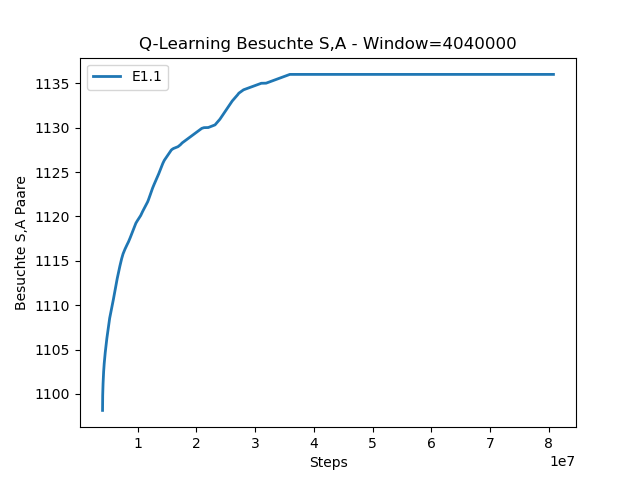
\includegraphics[height=5.5cm]{img/plots/exp-1/visited_800k.png}
  \caption{SA-Paare – Zufällige Actions 800'000 Episoden}
      \label{fig:visited_800k}
\end{figure}
Um sicherzustellen, dass sämtliche möglichen State-Action-Paare besucht werden, wurde ein rein explorativer Agent für 800'000 Episoden aufgeführt. In Abbildung \ref{fig:visited_800k} ist ersichtlich, wie nach ungefähr 400'000 Episoden 1136 State-Action-Paare besucht wurden. In der zweiten Hälfte wurden dabei keine weiteren States gefunden, woraus sich schliessen lässt, dass keine weiteren State-Action-Paare erreichbar sind. Um die Parameter zu prüfen, werden jeweils 50'000 Episoden durchgeführt. Diese garantieren nicht, dass jedes State-Action-Paar besucht wurde, da dies bei einem Agent, der zufällige Actions wählt, erst nach ungefähr 400'000 Episoden der Fall ist. Sie geben aber bereits einen hilfreichen Eindruck, welche Parameter besser geeignet sind. Die Policies mit den richtigen Parametern werden aber anschliessend mit 800'000 Episoden erlernt. Ausserdem wird überprüft, ob die 1136 State-Action-Paare erreicht wurden. 
\subsection{Exploration}
Als Erstes wird die Exploration untersucht. Der Explorationswert $\epsilon$ wird zu Beginn bei 1 festgelegt und über die Zeit mit einem Faktor, dem Epsilon-Verfall, verringert, bis ein Minimum von 0.05 erreicht wird. Dadurch soll sichergestellt werden, dass am Ende immer noch eine 5-prozentige Chance besteht, dass eine zufällige Action gewählt wird. Es werden unterschiedliche Werte für den Epsilon-Verfall gewählt und untersucht. Hierbei wird versucht, möglichst kurz zu explorieren, aber sicherzustellen, dass eine optimale Policy gefunden wird und der Agent nicht bei einem lokalen Optimum verbleibt. Dazu wird verglichen, nach wie vielen Steps wie viele States besucht wurden. Dabei wird im Durchgang 1.5 ein Verfall von 1 gewählt, um so ein rein exploratives Vorgehen zu erzwingen. Ein Parameter möglichst nah an 1, welcher noch genügend Episoden zum Optimieren übriglässt, wäre ideal. Folgende Parameter werden geprüft:
\begin{table}[H]%
\begin{tabularx}{\textwidth} { 
  | >{\raggedright\arraybackslash}X 
  | >{\raggedright\arraybackslash}X 
  | >{\raggedright\arraybackslash}X
  | >{\raggedright\arraybackslash}X|}
 \hline
  Durchgang &Discount-Factor $\gamma$ &Lernrate $\alpha$ &$\epsilon$-Verfall\\
\hline
 E1.1&	0.9	&0.5	&\textbf{0.9985}\\
 \hline
  E1.2&	0.9	&0.5	&\textbf{0.9990}\\
 \hline
  E1.3&	0.9	&0.5	&\textbf{0.9995}\\
 \hline
  E1.4&	0.9	&0.5	&\textbf{0.9999}\\
 \hline
  E1.5&	0.9	&0.5	&\textbf{1}\\
 \hline
\end{tabularx}
\caption{Experiment 1 – Epsilon-Verfall}
\end{table}%
\newpage
\subsection{Discount-Factor}
Der Discount-Factor $\gamma$ definiert, wie stark zukünftige Rewards gewertet werden. Ein \\ Discount-Factor von 0 bedeutet, dass der Agent ausschliesslich auf den aktuellen Reward achtet. Im Gegensatz dazu sagt ein Wert 1 aus, dass sämtliche zukünftigen Rewards berücksichtigt werden. Folgende Parameter werden geprüft:
\begin{table}[H]%
\begin{tabularx}{\textwidth} { 
  | >{\raggedright\arraybackslash}X 
  | >{\raggedright\arraybackslash}X 
  | >{\raggedright\arraybackslash}X
  | >{\raggedright\arraybackslash}X|}
 \hline
  Durchgang &Discount-Factor $\gamma$ &Lernrate $\alpha$ &$\epsilon$-Verfall\\
\hline
 G1.1&	\textbf{0.9}	&0.5	&0.999\\
 \hline
  G1.2&	\textbf{0.8}	&0.5	&0.999\\
 \hline
  G1.3&	\textbf{0.7}	&0.5	&0.999\\
 \hline
  G1.4&	\textbf{0.6}	&0.5	&0.999\\
 \hline
  G1.5&	\textbf{0.5}	&0.5	&0.999\\
 \hline
\end{tabularx}
\caption{Experiment 1 – Discount-Factor}
\end{table}%

\subsection{Lernrate}
Die Lernrate $\alpha$ definiert, wie schnell 
die Q-Values auf neue Erkenntnisse
angepasst werden. Ein Wert von 0 
bedeutet, es wird nichts dazugelernt, und der Wert 1 heisst, dass der komplette TD-Error ausgeglichen wird. Folgende Lernraten werden überprüft:
\begin{table}[H]%
\begin{tabularx}{\textwidth} { 
  | >{\raggedright\arraybackslash}X 
  | >{\raggedright\arraybackslash}X 
  | >{\raggedright\arraybackslash}X
  | >{\raggedright\arraybackslash}X|}
 \hline
  Durchgang &Discount-Factor $\gamma$ &Lernrate $\alpha$ &$\epsilon$-Verfall\\
\hline
 A1.1&	0.9	&\textbf{0.5}	&0.999\\
 \hline
  A1.2&	0.9	&\textbf{0.6}	&0.999\\
 \hline
  A1.3&	0.9	&\textbf{0.7}	&0.999\\
 \hline
  A1.4&	0.9	&\textbf{0.8}	&0.999\\
 \hline
  A1.5&	0.9	&\textbf{0.9}	&0.999\\
 \hline
\end{tabularx}
\caption{Experiment 1 – Lernrate}
\end{table}%

\newpage
\subsection{Messwerte}
Der Messwert, mit welchem die Policies verglichen werden, ist der Reward. Dazu wird der mittlere Reward der letzten 50 Episoden verwendet; ausserdem wird dieser Wert noch durch 100 dividiert, um somit den mittleren Step-Reward pro Episode zu erhalten. Der mittlere Step-Reward ist deshalb interessant, da man diesen mit einem optimalen Wert vergleichen kann. Es werden alle 4 Steps Aufträge generiert, und somit wäre ohne Lagerkosten pro Step ein Reward von 25 das Maximum.
Zuerst werden in einem direkten Vergleich die beiden Algorithmen gegenübergestellt. Dadurch soll ersichtlich sein, welcher Algorithmus einen höheren Reward erreicht und überprüft werden, ob sämtliche State-Action-Paare besucht wurden.
In einem zweiten Schritt wird nun noch die erlernte Policy der Algorithmen direkt auf einen Agent übertragen, welcher jeweils ohne Exploration die beste Action auswählt. Somit kann ein fairer Vergleich mit denselben Bestellungen angestellt werden. Dabei ist zu erwarten, dass die Policies ein konstantes Ergebnis über die Episoden erreichen, da mit nur einem Artikel kein Zufall im Environment vorhanden ist.
Die Werte in den Diagrammen werden, um die Übersichtlichkeit zu erhöhen, über eine bestimmte Anzahl an Werten, das sogenannte Window, gemittelt.
\smallskip\\
\begin{figure}[hb]
  \centering
  \href{https://github.com/benji24290/rl-warehouse/tree/experiment_1}{
\includegraphics[height=1.9cm]{img/qr/qrcode_exp1.jpeg}}
  \caption{Experiment 1 – Link}
\end{figure}
\newpage
\section{Resultate}
Im ersten Experiment, welches in \ref{sec:exp1-desc} definiert ist, wurde als Erstes die Exploration untersucht. Dabei konnte geprüft werden, welcher Epsilon-Verfall am besten geeignet ist. Der Wert 0.9999 aus Durchgang E1.4 erweist sich bei beiden Algorithmen als gut geeignet, da die State-Action-Paare am schnellsten erreicht werden und bereits ab 30'000 Episoden nur noch mit dem Minimum exploriert wird. Dadurch hat der Agent noch die restlichen Episoden Zeit, die Q-Values der State-Action-Paare zu optimieren. Bei 800'000 Episoden muss das entsprechende Epsilon angepasst werden, was gerundet ungefähr einem Epsilon-Verfall von 0.9999938 entspricht.
\begin{figure}[H]
\centering
  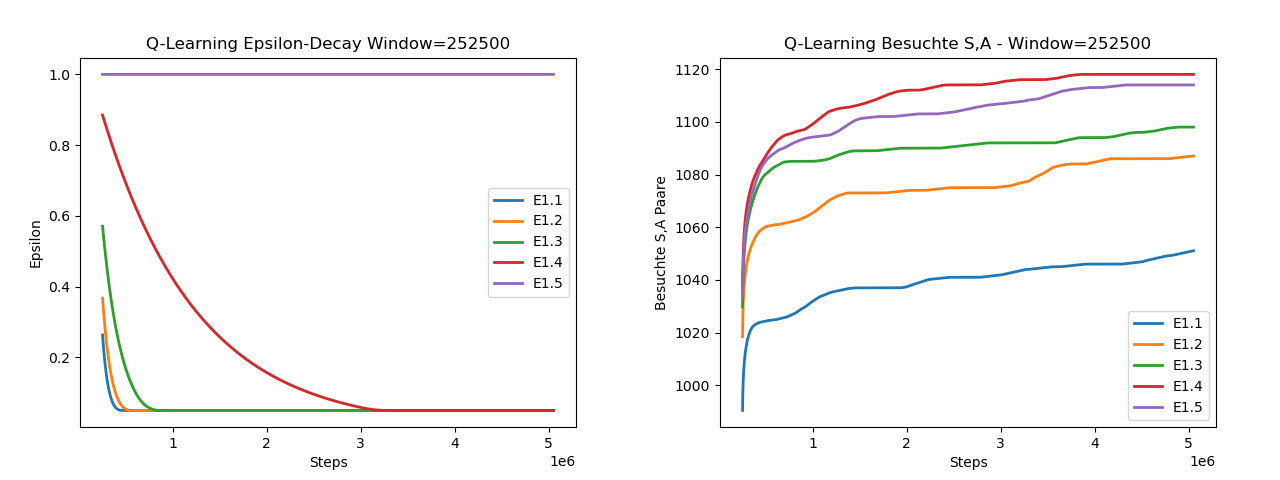
\includegraphics[height=5.5cm]{img/plots/exp-1/Exploration_Q.png}
  \caption{Experiment 1 – Exploration Q-Learning}
    \label{fig:e1-expl-q}
\end{figure} 
\begin{figure}[H]
\centering
  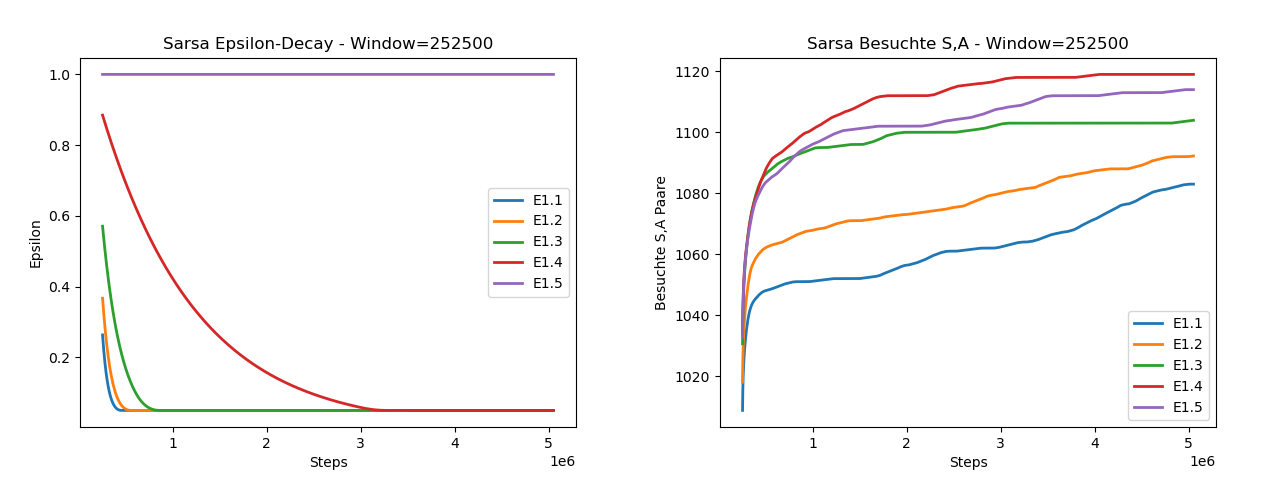
\includegraphics[height=5.5cm]{img/plots/exp-1/Exploration_Sarsa.png}
  \caption{Experiment 1 – Exploration Sarsa}
    \label{fig:e1-expl-q}
\end{figure} 

In Tabelle \ref{tab:e1-res-alpha} sind die Ergebnisse aus dem Parametervergleich für die Lernrate ersichtlich. Hierbei wurde jeweils der durchschnittliche Step-Reward der letzten 50 Episoden berechnet. Dabei ist erkennbar, dass die beiden Algorithmen jeweils mit unterschiedlichen Lernraten am besten performen. Für Q-Learning wird beim finalen Trainieren eine Lernrate von 0.9 und bei Sarsa 0.6 verwendet; diese haben in Tabelle \ref{tab:e1-res-alpha} jeweils den höchsten Step-Reward erzielt.
\begin{table}[H]%
\begin{tabularx}{\textwidth} { 
  | >{\raggedright\arraybackslash}X 
  | >{\raggedright\arraybackslash}X 
  | >{\raggedright\arraybackslash}X
  | >{\raggedright\arraybackslash}X|}
 \hline
  Durchgang &Lernrate &Q-Learning &Sarsa\\
\hline
 A1.1&0.5	&16.18 &14.71\\
 \hline
  A1.2&0.6	&18.26 &\textbf{17.22}\\
 \hline
  A1.3&0.7	&18.14 &15.16\\
 \hline
  A1.4&0.8	&18.02 &13.14\\
 \hline
  A1.5&0.9 &\textbf{19.42} &10.84\\
 \hline
\end{tabularx}
\caption{Experiment 1 – Resultate Lernrate}
\label{tab:e1-res-alpha}
\end{table}%

Zuletzt wurde der Discount-Factor überprüft. Dabei wurde auch der durchschnittliche Step-Reward aus den letzten 50 Episoden errechnet. Aus Tabelle \ref{tab:e1-res-gamma} wird ersichtlich, dass Q-Learning mit einem Gamma von 0.8 und Sarsa mit einem Gamma von 0.6 am besten performen.

\begin{table}[H]%
\begin{tabularx}{\textwidth} { 
  | >{\raggedright\arraybackslash}X 
  | >{\raggedright\arraybackslash}X 
  | >{\raggedright\arraybackslash}X
  | >{\raggedright\arraybackslash}X|}
 \hline
  Durchgang &Discount-Factor &Q-Learning &Sarsa\\
\hline
 G1.1&0.9	&16.18 &14.71\\
 \hline
  G1.2&0.8	&\textbf{17.45} &17.26\\
 \hline
  G1.3&0.7	&16.47 &16.01\\
 \hline
  G1.4&0.6	&18.02 &\textbf{18.43}\\
 \hline
  G1.5&0.5 &15.55 &17.93\\
 \hline
\end{tabularx}
\caption{Experiment 1 – Resultate Discount-Factor}
\label{tab:e1-res-gamma}
\end{table}%
\newpage
Nach den drei Durchgängen, in denen jeweils die besten Parameter für die beiden Algorithmen gewählt wurden, wird nun während 800'000 Episoden versucht, eine optimale Policy zu erlernen. Dabei ist in Abbildung \ref{fig:e1-train} zu sehen, dass Q-Learning einen höheren durchschnittlichen Reward erreicht als Sarsa. Der transparente Bereich zeigt die Varianz des Rewards. Der $TDError^2$, welcher aus Abbildung \ref{fig:e1-train} hervorgeht, hat bei beiden Algorithmen nach etwa 500'000 Episoden konvergiert. Der Grund dafür ist das Epsilon, welches – wie Abbildung \ref{fig:e1-expl-both} zeigt – nach dieser Anzahl an Episoden auf dem Minimum von 0.05 angekommen ist. Ausserdem erkennt man, wie Q-Learning, im Gegensatz zu Sarsa, die Anzahl der erreichbaren State-Action-Kombinationen bereits kurz vor 600'000 Episoden (Abbildung \ref{fig:e1-expl-both}) erreicht hat.
\begin{figure}[H]
  \centering
  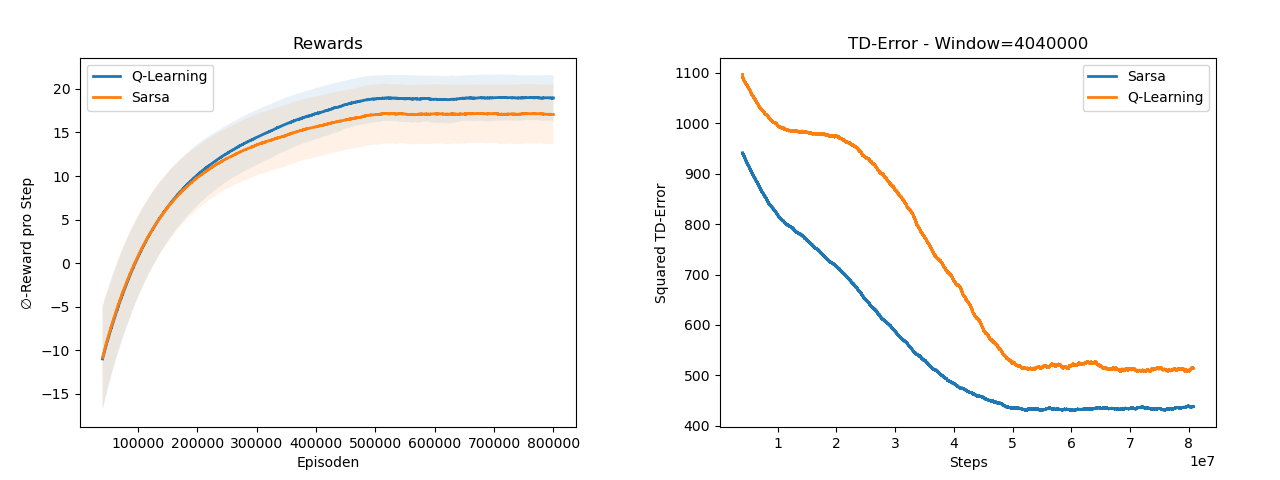
\includegraphics[height=5.5cm]{img/plots/exp-1/train.png}
  \caption{Experiment 1 – Reward und TD-Error}
    \label{fig:e1-train}
\end{figure} 
\begin{figure}[H]
  \centering
  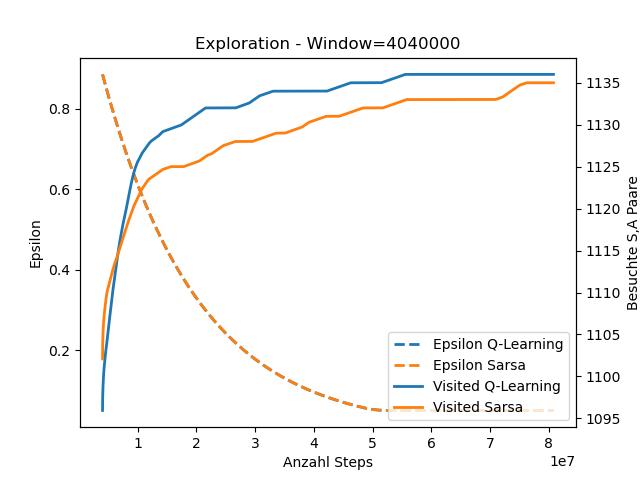
\includegraphics[height=5.5cm]{img/plots/exp-1/both_exploration.png}
  \caption{Experiment 1 – Exploration}
    \label{fig:e1-expl-both}
\end{figure}
In der folgenden Abbildung \ref{fig:e1-reward-freq} ist ersichtlich, wie oft ein gewisser Reward in der jeweiligen Episode verteilt wurde. Für negative Rewards wurde die Anzahl invertiert. Dabei ist zu erkennen, wie die Algorithmen die negativen Rewards, wie die für das Stornieren, für eine volle Ankunft oder eine falsche Auslieferung minimieren. Auch die Lagerkosten werden versucht auf das Nötigste zu minimieren. Nur die gelungenen Auslieferungen pro Episode haben mit steigender Anzahl an Episoden zugenommen.
\begin{figure}[H]
  \centering
  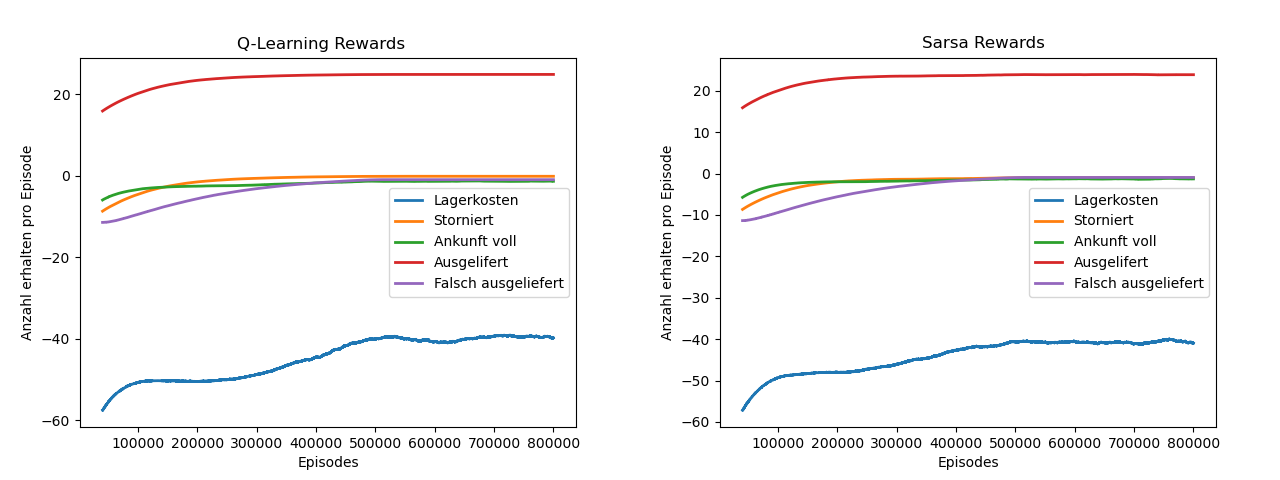
\includegraphics[height=5.3cm]{img/plots/exp-1/reward_frequency.png}
  \caption{Experiment 1 – Vorkommen der Rewards pro Step (Window = 40'400)}
    \label{fig:e1-reward-freq}
\end{figure}
Mit dem erfolgreichen Trainieren der Policies steht nun eine Q-Matrix zur Verfügung, die an einen Greedy-Agent übergeben wird. Dieser Agent wählt ausschliesslich die Action, welche den höchsten Q-Value für einen gegebenen State aufweist. Wie erwartet, ist in Abbildung \ref{fig:e1-comp-policies} zu erkennen, dass die Policies über die 1000 Episoden jeweils denselben Reward erzielen. Das ist korrekt, da in Experiment 1 nur ein Artikel und somit in jeder Episode dasselbe Sample an Aufträgen entsteht.
\begin{figure}[H]
  \centering
  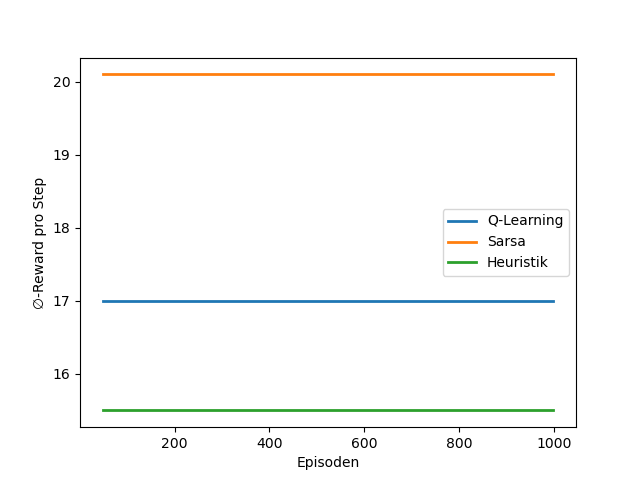
\includegraphics[height=5.2cm]{img/plots/exp-1/Compare.png}
  \caption{Experiment 1 – Vergleich der Policies}
    \label{fig:e1-comp-policies}
\end{figure}

In diesem Experiment hat Sarsa den mittleren Step-Reward der heuristischen Policy um 30 Prozent übertroffen (Tabelle \ref{tab:e1-res-poli}).
\begin{table}[H]%
\begin{tabularx}{\textwidth} { 
  | >{\raggedright\arraybackslash}l 
  | >{\raggedright\arraybackslash}X 
  | >{\raggedright\arraybackslash}X
  | >{\raggedright\arraybackslash}X|}
 \hline
  Policy &Q-Learning &Sarsa &Heuristik\\
\hline
 Ø-Step-Reward&17.0	&20.1 &15.5\\
 \hline
  Vergleich zur Heuristik&+9.7\%	&+29.7\% &+0\%\\
 \hline
\end{tabularx}
\caption{Experiment 1 – Resultate Policies}
\label{tab:e1-res-poli}
\end{table}%

In den folgenden Abbildungen \ref{fig:e1-pol-heu}, \ref{fig:e1-pol-q} und \ref{fig:e1-pol-sarsa} wurde für jeden Agent dieselbe Episode ausgewählt und die erreichten Rewards sowie der State dieser Episode wurden dargestellt. Diese Darstellungen ermöglichen es, die Unterschiede der Agents besser aufzuzeigen.
Abbildung \ref{fig:e1-pol-heu} zeigt die Rewards der Heuristik für eine Episode. Wie man erkennen kann, verpasst diese Policy jede 5. Bestellung. Dieses Resultat ist nachvollziehbar, denn die definierte Heuristik hält nur ein Exemplar pro Artikel auf Lager und das Bestellen bis zum Ausliefern dauert 5 Steps. Es werden jedoch alle 4 Steps Aufträge generiert.

\begin{figure}[H]
  \centering
  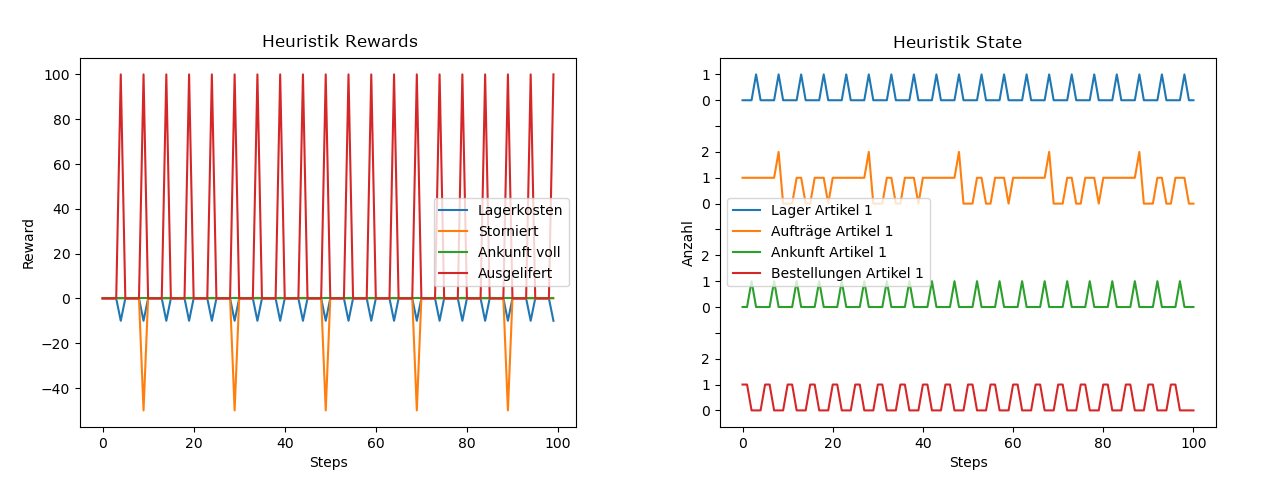
\includegraphics[height=5.5cm]{img/plots/exp-1/heu-rew-state.png}
  \caption{Experiment 1 – Rewards und States aus einer Episode Heuristik}
    \label{fig:e1-pol-heu}
\end{figure}

\newpage
Wie in Abbildung \ref{fig:e1-pol-q} erkennbar, hat die Q-Learning-Policy versucht, die Lagerplätze durch den Wareneingang zu ersetzen, da dieser im Environment keine Kosten generiert. Da aber zu viele Artikel im Eingang sind, wird trotzdem ein negativer Reward verteilt. 

\begin{figure}[H]
  \centering
  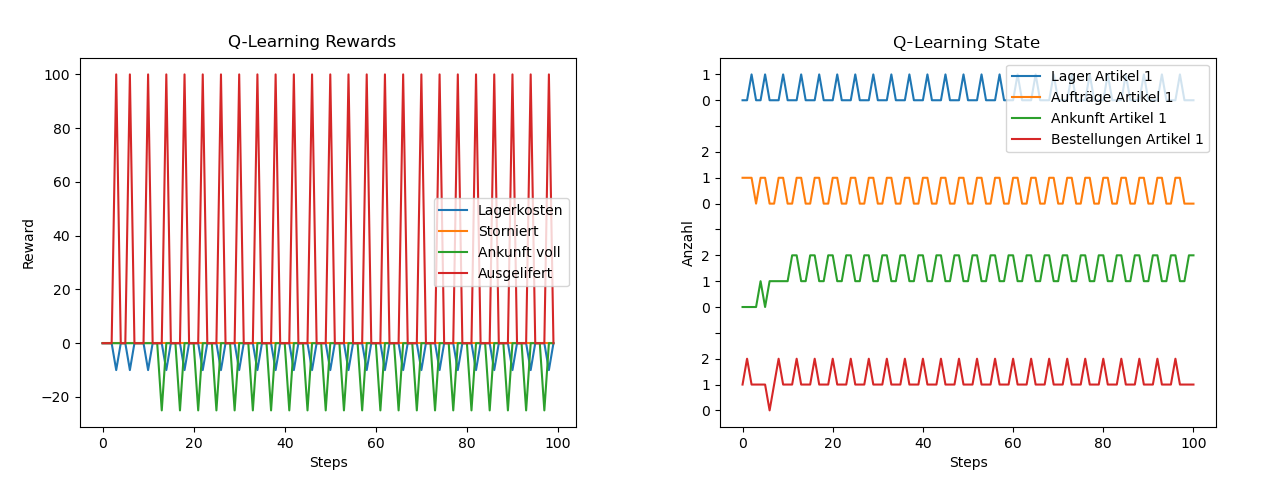
\includegraphics[height=5.5cm]{img/plots/exp-1/q-rew-state.png}
  \caption{Experiment 1 – Rewards und States aus einer Episode Q-Learning}
    \label{fig:e1-pol-q}
\end{figure}
Sarsa hingegen hat gelernt, dass nur zu Beginn zwei Bestellungen nacheinander vorkommen und bestellt diese demensprechend (Abbildung \ref{fig:e1-pol-sarsa}). Dieses Vorgehen entspricht einem Overfitting, was in diesem Fall das Auswendiglernen einer bestimmten Sequenz bedeutet. Da das Environment aber immer gleich bleibt und keine zufälligen Abläufe stattfinden, ist das in diesem Fall die beste Policy.
\begin{figure}[H]
  \centering
  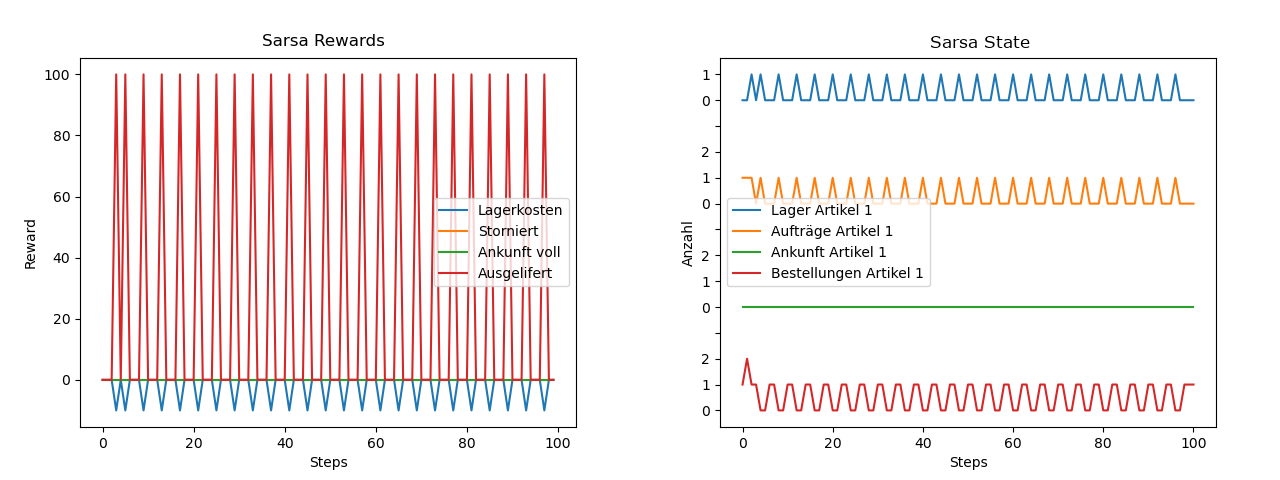
\includegraphics[height=5.5cm]{img/plots/exp-1/sarsa-rew-state.png}
  \caption{Experiment 1 – Rewards und States aus einer Episode Sarsa}
    \label{fig:e1-pol-sarsa}
\end{figure}
\chapter{Experiment 2}
Bei der zweiten Forschungsfrage soll das Verhalten der Performanz bei einer steigenden Komplexität im Environment überprüft werden. 
\section{Beschreibung}
Um das Verhalten der Performanz bei einer höheren Komplexität zu überprüfen, wird das Environment um einen Artikel erweitert. Diese Erweiterung hört sich nach einer nicht besonders grossen Komplexitätssteigerung an. Um den Unterschied aufzuzeigen, können von beiden Environments die maximal möglichen State-Action-Kombinationen berechnet werden. 
Eine Observation aus dem State-Space besteht aus den neun in \autoref{sec:state-space} beschriebenen Features, wobei jedes dieser Features 0 für leer, 1 für Artikel 1 und 2 für Artikel 2 annehmen kann. 

\begin{align}
    &States\ =\ {(Artikel+1)}^{Features} \nonumber\\
&Actions\ =\ Artikel+3
\end{align}

\begin{table}[H]%
\begin{tabularx}{\textwidth} { 
  | >{\raggedright\arraybackslash}X 
  | >{\raggedright\arraybackslash}l 
  | >{\raggedright\arraybackslash}X
  | >{\raggedright\arraybackslash}X|}
 \hline
  Environment &States-Kombinationen &Actions &SA-Kombinationen\\
\hline
 1 Artikel&$2^9$ = 512  	&5 &2’560\\
 \hline
  2 Artikel&$3^9$ = 19’683  	&6 &118’098\\
 \hline
\end{tabularx}
\caption{Experiment 1 – Resultate Policies}
\label{tab:e1-res-gamma}
\end{table}%
Diese Kombinationen sind theoretisch möglich; davon sind aber nicht alle erreichbar, da es gewisse Regeln im Environment gibt. Der Agent kennt diese Regeln allerdings nicht. Des Weiteren spielt die Reihenfolge, ob ein Artikel im Lager auf Platz 0, 1 oder 2 vorhanden ist, keine Rolle. Auch diese Information ist dem Agent nicht bewusst und er müsste alle 3 Varianten kennenlernen.
Da in diesem Experiment nun zwei mögliche Artikel verfügbar sind, hat die Häufigkeit der Artikel nun einen Einfluss. Für dieses Experiment wird ein \emph{Artikel 1} mit der Häufigkeit von 0.2 und einer mit der Häufigkeit von 0.8 definiert. Dadurch werden im Durchschnitt vier Mal so viele Aufträge mit dem \emph{Artikel 2} generiert.
\subsection{Parameter}
Die relevanten Parameter für dieses Experiment entsprechen denen aus Experiment 1. Die Anzahl an Episoden ist in diesem Experiment zu Beginn auch auf einen Wert definiert. Es werden pro Durchgang jeweils 50’000 Episoden durchgeführt.\\
Die Durchgänge werden mit den folgenden Parametern ausgeführt:\\
\begin{table}[H]%
\begin{tabularx}{\textwidth} { 
  | >{\raggedright\arraybackslash}X 
  | >{\raggedright\arraybackslash}X 
  | >{\raggedright\arraybackslash}X
  | >{\raggedright\arraybackslash}X|}
 \hline
  Durchgang &Discount-Factor $\gamma$ &Lernrate $\alpha$ &$\epsilon$-Verfall\\
\hline
 E2.1&	0.9	&0.5	&\textbf{0.9985}\\
 \hline
  E2.2&	0.9	&0.5	&\textbf{0.9990}\\
 \hline
  E2.3&	0.9	&0.5	&\textbf{0.9995}\\
 \hline
  E2.4&	0.9	&0.5	&\textbf{0.9999}\\
 \hline
  E2.5&	0.9	&0.5	&\textbf{1}\\
 \hline
  G2.1&	\textbf{0.9}	&0.5	&0.999\\
 \hline
  G2.2&	\textbf{0.8}	&0.5	&0.999\\
 \hline
  G2.3&	\textbf{0.7}	&0.5	&0.999\\
 \hline
  G2.4&	\textbf{0.6}	&0.5	&0.999\\
 \hline
  G2.5&	\textbf{0.5}	&0.5	&0.999\\
 \hline
  A2.1&	0.9	&\textbf{0.5}	&0.999\\
 \hline
  A2.2&	0.9	&\textbf{0.6}	&0.999\\
 \hline
  A2.3&	0.9	&\textbf{0.7}	&0.999\\
 \hline
  A2.4&	0.9	&\textbf{0.8}	&0.999\\
 \hline
  A2.5&	0.9	&\textbf{0.9}	&0.999\\
 \hline
\end{tabularx}
\caption{Experiment 2 – Parameter}
\end{table}%
\subsection{Messwerte}
Auch bei diesem Experiment werden die Resultate dem durchschnittlichen Step-Reward pro Episode gegenübergestellt. Die Algorithmen werden mithilfe desselben Vorgehens aus Experiment 1 untersucht und miteinander verglichen. Auch hier wird anschliessend wieder mit einem Agent verglichen, der ausschliesslich die Action mit dem grössten Q-Value, der Greedy-Policy, wählt. Dabei sollte eine Varianz in den Resultaten der Policies zu erkennen sein, da nun Aufträge mit zufälligen Artikeln erstellt werden.
\smallskip\\
\begin{figure}[hb]
  \centering
  \href{https://github.com/benji24290/rl-warehouse/tree/experiment_2}{
\includegraphics[height=1.9cm]{img/qr/qrcode_exp2.jpeg}}
  \caption{Experiment 2 – Link}
\end{figure}

%RESULTS
\section{Resultate}
Auch im zweiten Experiment, welches in Abschnitt \ref{fig:e2-expl} definiert ist, wurde als Erstes die Exploration untersucht. Das Verhalten von Epsilon hat sich zum vorherigen Experiment nicht verändert, da das Epsilon nicht mit der Anzahl an State-Action-Paaren, sondern mit der Anzahl an Episoden verringert wird. Aufgrund der gestiegenen Anzahl möglicher State-Action-Kombinationen werden in derselben Anzahl an Episoden deutlich mehr State-Action-Paare besucht. 
\begin{figure}[H]
  \centering
  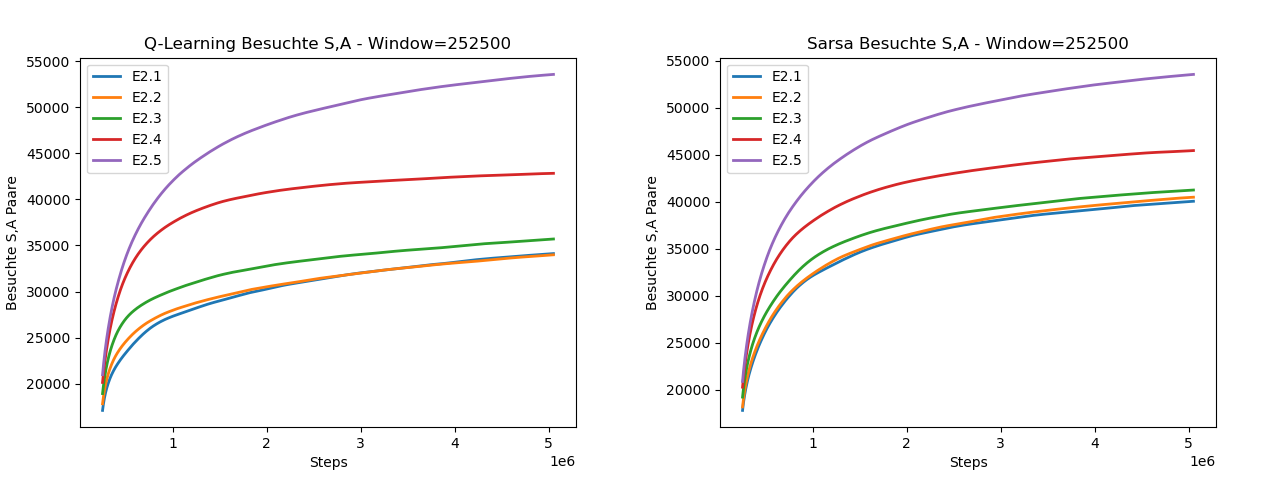
\includegraphics[height=5.5cm]{img/plots/exp-2/visited.png}
  \caption{Experiment 2 – Besuchte SA-Paare}
    \label{fig:e2-expl}
\end{figure} 
Als Zweites wurden die Lernraten untersucht. Dabei haben die Agents die in Tabelle \ref{tab:e2-res-alpha-1} ersichtlichen Resultate erzielt. Zu sehen ist, dass mit sinkender Lernrate der Reward weiter gestiegen ist. Aus diesem Grund wurde noch ein zweiter Durchgang gestartet, welcher kleinere Lernraten untersucht.
\begin{table}[H]%
\begin{tabularx}{\textwidth} { 
  | >{\raggedright\arraybackslash}X 
  | >{\raggedright\arraybackslash}X 
  | >{\raggedright\arraybackslash}X
  | >{\raggedright\arraybackslash}X|}
 \hline
  Durchgang &Lernrate &Q-Learning &Sarsa\\
\hline
 A2.1&0.5	&\textbf{3.72} &\textbf{3.05}\\
 \hline
  A2.2&0.6	&-1.16 &-2.00\\
 \hline
  A2.3&0.7	&-1.52 &-3.27\\
 \hline
  A2.4&0.8	&-4.77 &-8.61\\
 \hline
  A2.5&0.9 &-9.35 &-14.40\\
 \hline
\end{tabularx}
\caption{Experiment 2 – Resultate Lernrate 1}
\label{tab:e2-res-alpha-1}
\end{table}%

Beim zweiten Durchgang wurden die folgenden Resultate (Tabelle \ref{tab:e2-res-alpha-2}) erzielt. Die Annahme wurde bestätigt, wodurch in diesem Durchgang für beide Algorithmen eine bessere Lernrate mit dem Wert 0.1 gefunden werden konnte.

\begin{table}[H]%
\begin{tabularx}{\textwidth} { 
  | >{\raggedright\arraybackslash}X 
  | >{\raggedright\arraybackslash}X 
  | >{\raggedright\arraybackslash}X
  | >{\raggedright\arraybackslash}X|}
 \hline
  Durchgang &Lernrate &Q-Learning &Sarsa\\
\hline
 A2.6&0.4	&3.44 &0.69\\
 \hline
  A2.7&0.3	&2.61 &3.62\\
 \hline
  A2.8&0.2	&6.50 &5.46\\
 \hline
  A2.9&0.1	&\textbf{6.62} &\textbf{6.33}\\
 \hline
  A2.10&0.01 &3.60 &2.67\\
 \hline
\end{tabularx}
\caption{Experiment 2 – Resultate Lernrate 2}
\label{tab:e2-res-alpha-2}
\end{table}%
Als letzter Parameter wurde hier der Discount-Factor untersucht. Wie in Tabelle \ref{tab:e2-res-gamma} ersichtlich, hat sich ein Gamma von 0.9 für beide Algorithmen als der beste getestete Wert erwiesen.

\begin{table}[H]%
\begin{tabularx}{\textwidth} { 
  | >{\raggedright\arraybackslash}X 
  | >{\raggedright\arraybackslash}X 
  | >{\raggedright\arraybackslash}X
  | >{\raggedright\arraybackslash}X|}
 \hline
  Durchgang &Discount-Factor &Q-Learning &Sarsa\\
\hline
 G2.1&0.9	&\textbf{3.72} &\textbf{3.05}\\
 \hline
  G2.2&0.8	&-0.28 &-5.76\\
 \hline
  G2.3&0.7	&-4.84 &-13.13\\
 \hline
  G2.4&0.6	&-9.98 &-15.34\\
 \hline
  G2.5&0.5 &-10.45 &-13.14\\
 \hline
\end{tabularx}
\caption{Experiment 2 – Resultate Discount-Factor}
\label{tab:e2-res-gamma}
\end{table}%

Nach den vier Durchgängen, in welchen die besten Parameter gesucht wurden, werden nun mit beiden Algorithmen erneut die Policies erlernt. In Abbildung \ref{fig:e2-train} ist zu erkennen, dass dieses Mal Q-Learning zu einem kleineren TD-Error konvergiert. Die Rewards beim Lernen befinden sich bei beiden Algorithmen in einem ähnlichen Bereich. 
\begin{figure}[H]
  \centering
  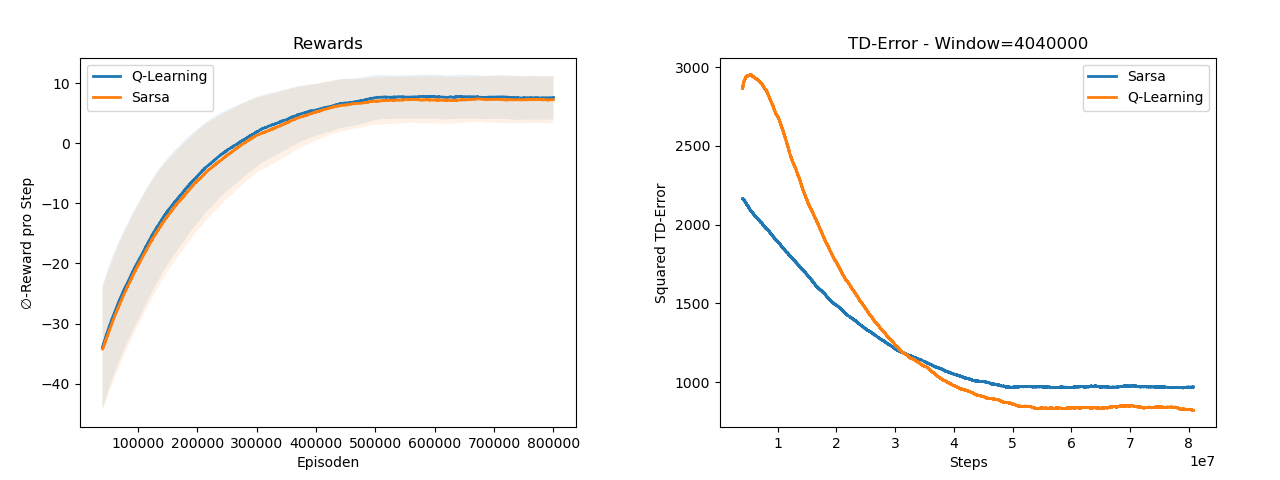
\includegraphics[height=5.5cm]{img/plots/exp-2/rew&td.png}
  \caption{Experiment 2 – Reward und TD-Error}
    \label{fig:e2-train}
\end{figure} 
Die besuchten State-Action-Paare sind im Verhältnis zur maximalen Anzahl möglicher Kombinationen dem ersten Experiment äußerst ähnlich. 
\begin{figure}[H]
  \centering
  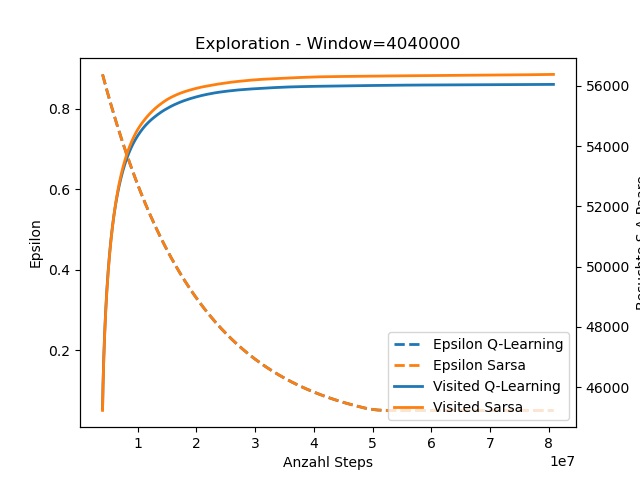
\includegraphics[height=5.5cm]{img/plots/exp-2/both_exploration.png}
  \caption{Experiment 2 – Exploration}
    \label{fig:e2-expl-both}
\end{figure}
\newpage
Bei den vorgekommenen Rewards pro Episode (Abbildung \ref{fig:e2-reward-freq}) haben beide Agents erneut gelernt, negative Rewards wie eine stornierte Bestellung und eine volle Ankunft zu vermeiden. Im Vergleich zum ersten Experiment sind aber die Lagerkosten deutlich gestiegen. Dies ist ein gutes Zeichen, denn nun kann der Agent nicht mehr genau einen Step vor der Bestellung den gewünschten Artikel bestellen, da dieser probabilistisch nach der Häufigkeit gewählt wird.
\begin{figure}[H]
\centering
  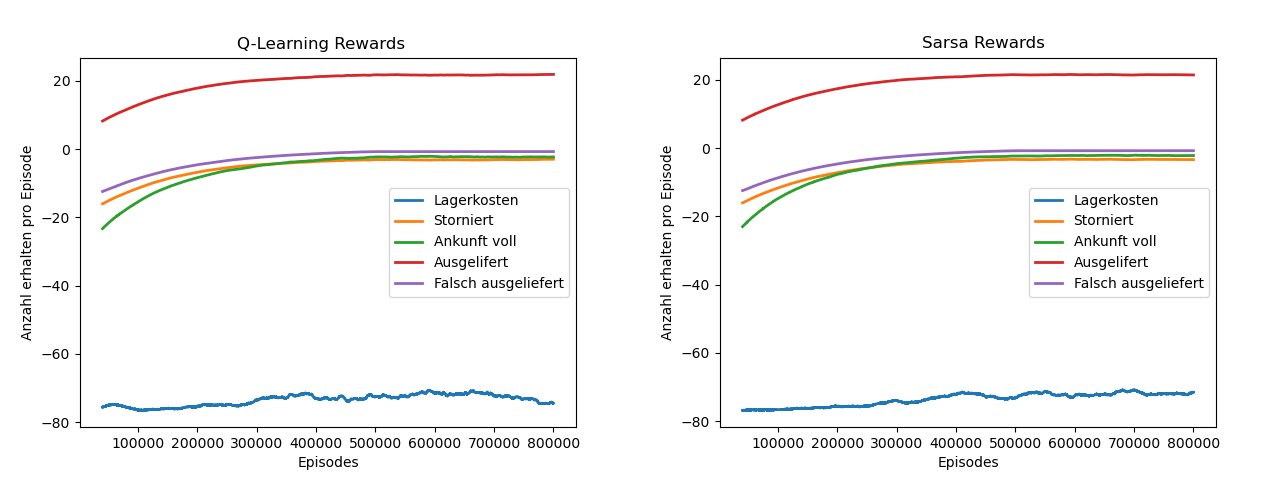
\includegraphics[height=5.5cm]{img/plots/exp-2/reward_count_episodes.png}
  \caption{Experiment 2 – Vorkommen der Rewards pro Step (Window = 40'400)}
    \label{fig:e2-reward-freq}
\end{figure}

Die erlernten Policies konnten im direkten Vergleich mit der Heuristik erneut bessere Resultate erzielen (Abbildung \ref{fig:e2-comp-policies}). Des Weiteren ist nun im Gegensatz zum ersten Experiment eine Varianz ersichtlich, da nun Artikel zufällig sind. 
\begin{figure}[H]
\centering
  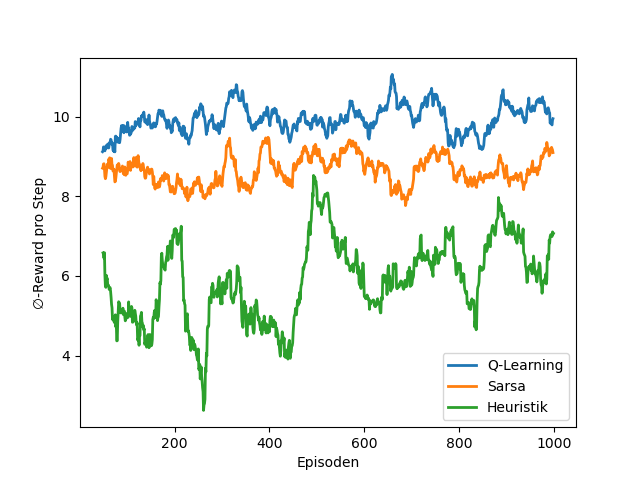
\includegraphics[height=5.5cm]{img/plots/exp-2/s_rewards.png}
  \caption{Experiment 2 – Vergleich der Policies}
    \label{fig:e2-comp-policies}
\end{figure}
\newpage
Erneut haben die Policies, die durch Reinforcement Learning erlernt wurden, die der Heuristik übertroffen. Q-Learning hat dabei den durchschnittlichen Step-Reward um 67 Prozent übertroffen (Tabelle \ref{tab:e2-policies}).
\begin{table}[H]%
\begin{tabularx}{\textwidth} { 
  | >{\raggedright\arraybackslash}l 
  | >{\raggedright\arraybackslash}X 
  | >{\raggedright\arraybackslash}X
  | >{\raggedright\arraybackslash}X|}
 \hline
  Policy &Q-Learning &Sarsa &Heuristik\\
\hline
 Ø-Step-Reward&9.92	&8.66 &5.93\\
 \hline
  Vergleich zur Heuristik&+67.3\%	&+46.0\% &+0\%\\
 \hline
\end{tabularx}
\caption{Experiment 2 – Resultate Policies}
\label{tab:e2-policies}
\end{table}%

Die folgenden Abbildungen stellen erneut die Rewards und die States aus einer Episode dar. In der Abbildung \ref{fig:e2-pol-heu} ist ersichtlich, wie die Policy der Heuristik fast durchgehend einen Artikel 1 auf Lager hat. Das ist nachvollziehbar, da die Heuristik versucht, jeweils mindestens einen Artikel im Lager zu halten, damit keine Lieferfrist für einen Auftrag abläuft. Daher sind die Lagerkosten im Vergleich zu den beiden durch Reinforcement Learning erlernten Strategien höher.

\begin{figure}[H]
\centering
  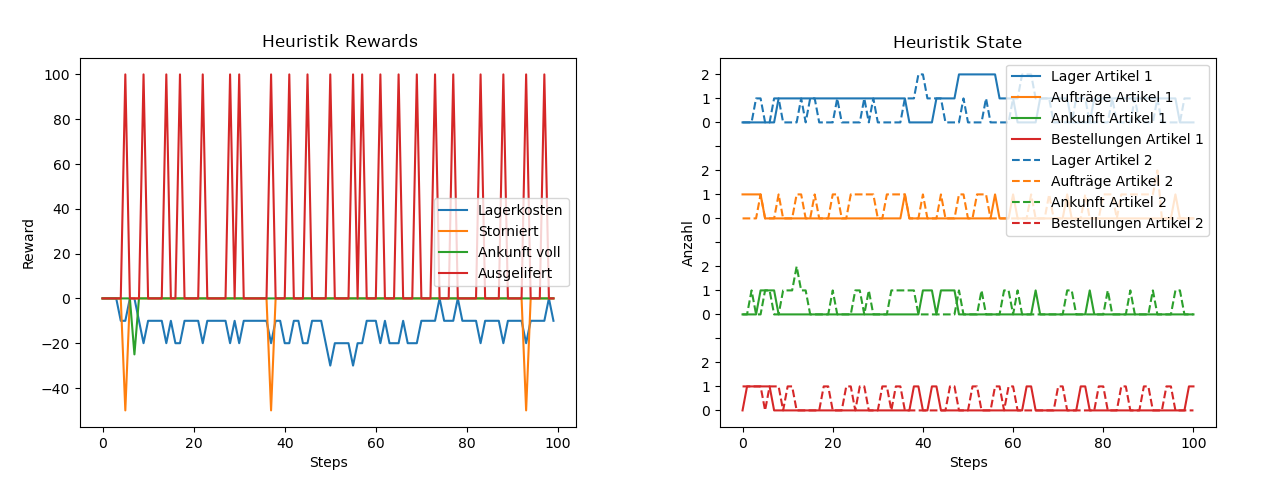
\includegraphics[height=5.5cm]{img/plots/exp-2/heu-rew-state.png}
  \caption{Experiment 2 – Rewards und States aus einer Episode Heuristik}
    \label{fig:e2-pol-heu}
\end{figure}
\newpage
Bei Q-Learning ist in Abbildung \ref{fig:e2-pol-q} erneut zu erkennen, dass die Ankunft benutzt wird, um Lagerkosten einzusparen. Allerdings gelingt es der Policy nicht, ein Überfüllen der Ankunft zu verhindern und daher bekommt sie drei Mal einen negativen Reward dafür. Dafür sind die Lagerkosten um einiges geringer, da nie drei Artikel im Lager sind. 

\begin{figure}[H]
\centering
  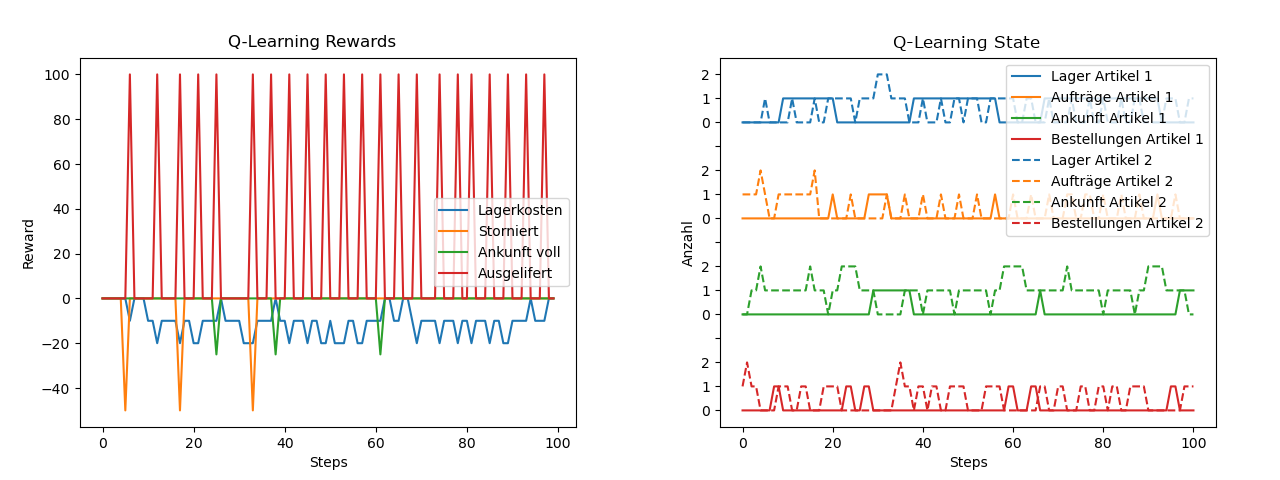
\includegraphics[height=5.5cm]{img/plots/exp-2/q-rew-state.png}
  \caption{Experiment 2 – Rewards und States aus einer Episode Q-Learning}
    \label{fig:e2-pol-q}
\end{figure}
In Abbildung \ref{fig:e2-pol-sarsa} sieht man, wie es Sarsa gelingt, die Ankunft sinnvoll zu verwenden, ohne dass die Ankunft ein Mal überfüllt wird. 
\begin{figure}[H]
    \centering
  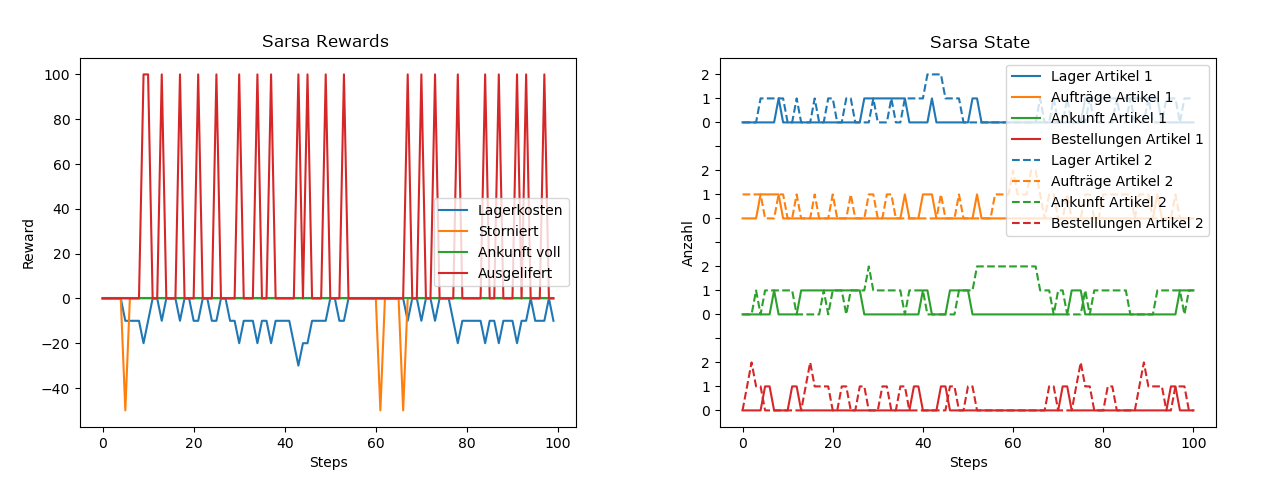
\includegraphics[height=5.5cm]{img/plots/exp-2/sarsa-rew-state.png}
  \caption{Experiment 2 – Rewards und States aus einer Episode Sarsa}
    \label{fig:e2-pol-sarsa}
\end{figure}

\chapter{Diskussion}

Die Resultate aus Experiment 1 zeigen, dass es für Reinforcement Learning in dieser minimalen Umgebung durchaus möglich ist, eine gute Policy zu erlernen und die Performanz der heuristisch definierten Policy zu übertreffen. Die durch Sarsa erlernte Policy hat dabei die Resultate der heuristischen Strategie um 30 Prozent übertroffen. Ausserdem hat der Q-Learning-Agent in diesem Experiment eine Policy erlernt, welche beim Erstellen des Environments nicht so eingeplant wurde. Der Agent hat festgestellt, dass Artikel in der Ankunft keine Lagerkosten generieren und dies dementsprechend mit mittlerem Erfolg genutzt. Dabei lässt sich die erste Forschungsfrage mit der Begrenzung auf das untersuchte Environment folgendermassen beantworten: Die Performanz, der durch Reinforcement Learning erlernten Strategie, übertrifft die der heuristischen Strategie.
Im zweiten Experiment wurde die Komplexität erhöht. Dabei konnte erneut die Performanz der Heuristik übertroffen werden. Die durch Q-Learning erlernte Policy erreichte einen durchschnittlichen Step-Reward der 67 Prozent höher war als der der Heuristik. Des Weiteren ist aber deutlich zu erkennen, dass durch das Wachstum des State-Action-Spaces eine höhere Anzahl an Episoden nötig war, um alle State-Action-Paare zu besuchen. Die zweite Forschungsfrage kann aufgrund dieser Ergebnisse wie folgt beantwortet werden: Die Performanz, der durch Reinforcement Learning erlernten Strategie, konnte die der heuristischen Strategie übertreffen. Dabei kann jedoch nicht auf ein reelles Lager generalisiert werden – dazu wurden zu wenige Artikel und Lagerplätze initialisiert. Eine Erweiterung um einen Artikel hat eine hohe Auswirkung auf den State. Die Information, welcher Artikel auf Lager ist, wird benötigt, um festzustellen, welche Artikel öfter bestellt werden. Eine Möglichkeit, die Komplexität drastisch zu verringern, wäre diese: Die States vom Environment werden auf 0 und 1 reduziert, wobei 1 bedeutet, es ist ein Artikel im Lager, in der Ankunft oder wurde soeben bestellt. Die Information über die Häufigkeit könnte mit einem Array, welches aus den letzten $n$ bestellten Artikel besteht, gespeichert werden.
Die in dieser Arbeit erzielten Ergebnisse dienen zur Grundlage und bieten als Artefakt ein erweiterbares Environment, welches mit geringem Aufwand weiter skaliert werden kann. Die nächste sinnvolle Untersuchung wäre eine Verkleinerung des State-Spaces. Ausserdem sollten weiterführende Algorithmen, welche sich in komplexeren Environments beweisen können – wie in den Atari-Spielen \cite{mnih2013playing} – verwendet werden. So wird häufig mit Deep Q-Learning ein Neuronales Netz erstellt anstatt einer Q-Matrix, welches besser auf unbesuchte State-Action-Paare generalisieren kann.
Ein Einsatz in einem reellen Lager könnte erst nach weiteren Untersuchungen abschliessend abgeschätzt werden. 


\listoffigures

\listoftables



\bibliography{thesis.bib}
\bibliographystyle{ieeetr}

\newpage

\appendix
\chapter{Anhang}
\label{sec:Anhang}
\section{Berechnung MDP - State-Values}
\label{appendix:state-values}
\begin{align}
&\gamma=1\nonumber\\
&\textbf{KB-NV} \nonumber\\
&v_*(KBNV) =\gamma *( P(KBNV)* v_*(KBNV)+ P(BT1NV)* v_*(BT1NV))+R(A1) \nonumber \\
&v_*(KBNV)= 1/2x +  9.5 -1= x \nonumber\\
&v_*(KBNV)= 17\\
&\textbf{KB-V} \nonumber\\
&v_*(KBV)= \gamma *(P(KBV)* v_*(KBV)+ P(BT1V)* v_*(BT1V)) + R(A1) \nonumber \\
&v_*(KBV)= 1/2x +  10-2 = x \nonumber\\
&v_*(KBV)= 16\\
&\textbf{BT1-V} \nonumber\\
&v_*(BT1V)= \gamma *(P(A)* v_*(A)) + R(A3) \nonumber \\
&v_*(BT1V)= 0 +20 = 20\\
&\textbf{BT1-NV} \nonumber\\
&v_*(BT1NV) = \gamma *(P(BT2V)* v_*(BT2V))+R(A1) \nonumber \\
&v_*(BT1NV) = 20 -1= 19\\
&\textbf{BT2-V} \nonumber\\
&v_*(BT2V)= \gamma *(P(A)* v_*(A)) + R(A3) \nonumber \\
&v_*(BT2V)= 0 +20 = 20
\end{align}

\section{Berechnung MDP - Action-Values}
\label{appendix:action-values}
\begin{align}
&\gamma=1\nonumber\\
&\textbf{KB-NV} \nonumber\\
&q_*(KBNV,A1) = \gamma *(P(KBNV)* v_*(KBNV)+ P(BT1NV)* v_*(BT1NV))+R(A1) \nonumber \\
&q_*(KBNV,A1)= 8.5 +  9.5 -1= 17\\
&q_*(KBNV,A2) = \gamma *(P(KBV)* v_*(KBV)+ P(BT1V)* v_*(BT1V)) +R(KBNV, A2)\nonumber \\
&q_*(KBNV,A2)= 8 +  10 -1 = 17\\
&\textbf{KB-V} \nonumber\\
&q_*(KBV,A1) = \gamma *(P(KBV)* v_*(KBV)+ P(BT1V)* v_*(BT1V)) + R(A1) \nonumber \\
&q_*(KBV,A1)= 8 +  10-2 = 16\\
&\textbf{BT1-V} \nonumber\\
&q_*(BT1V,A3) = \gamma *(P(A)* v_*(A)) + R(A3) \nonumber \\
&q_*(BT1V,A3)= 0 +20 = 20\\
&\textbf{BT1-NV} \nonumber\\
&q_*(BT1NV,A1) = \gamma *(P(KBNV)* v_*(KBNV))+R(A1) \nonumber \\
&q_*(BT1NV,A1)= 17 -1= 16\\
&q_*(BT1NV,A2) = \gamma *(P(BT2V)* v_*(BT2V)) +R(A2)\nonumber \\
&q_*(BT1NV,A2)= 20 -1 = 19\\
&\textbf{BT2-V} \nonumber\\
&q_*(BT2V,A3) = \gamma *(P(A)* v_*(A)) + R(A3) \nonumber \\
&q_*(BT2V,A3)= 0 +20 = 20
\end{align}

\begin{appendix}


\chapter*{Selbstständigkeitserklärung}
Ich erkläre hiermit, dass ich diese Thesis selbständig verfasst 
und keine andern als die angegebenen Quellen benutzt habe. 
Alle Stellen, die wörtlich oder sinngemäss aus Quellen entnommen wurden, 
habe ich als solche kenntlich gemacht. Ich versichere zudem, dass ich bisher 
noch keine wissenschaftliche Arbeit mit gleichem oder ähnlichem Inhalt an der 
Fernfachhochschule Schweiz oder an einer anderen Hochschule eingereicht habe. 
Mir ist bekannt, dass andernfalls die Fernfachhochschule Schweiz zum Entzug 
des aufgrund dieser Thesis verliehenen Titels berechtigt ist.

\vspace{4cm}
\noindent
\hrule \ \\[-0.5ex]
Ort, Datum, Unterschrift
\end{appendix}

\end{document}


